% ESTE ES EL PAPER ESTUDIANDO LOS DOMINIOS DEL MAPA DE SPROTT EN PUNTO FIJO
% la idea es hacer una version de este paper para mandar a Chaos, Solitons and Fractals FI 1.222.
% otra posibilidad es mandarlo a Communications in Nonlinear Science and Numerical Simulation, Elsevier Science, ISSN 1007-5704, FI 2.88
\documentclass{elsart}
%%%%%%%%%%%%%%%% The amssymb package provides various useful mathematical symbols
\usepackage{amssymb}
\usepackage{amsmath}
%%%%%% Para los graficos:
\usepackage[pctex32]{graphics}
\usepackage{graphicx}
\graphicspath{{converted_graphics/}}
% la idea es hacer una version de este paper para mandar a Chaos, Solitons and Fractals FI 1.222.
% otra posibilidad es mandarlo a Communications in Nonlinear Science and Numerical Simulation, Elsevier Science, ISSN 1007-5704, FI 2.88

\begin{document}

\newcommand{\be}{\begin{equation}}
\newcommand{\ee}{\end{equation}}
\newcommand{\ben}{\begin{eqnarray}}
\newcommand{\een}{\end{eqnarray}}
\newcommand{\nn}{\nonumber \\}
\newcommand{\ii}{\'{\i}}
\newcommand{\pp}{\prime}
\newcommand{\nd}{{\noindent}}

\begin{frontmatter}

% paper title
\title{Nontrivial behavior of the fixed-point version of $2D$-chaotic maps}
\author[mdp,CONICET]{Luciana De Micco},
\ead{lucianadm55@gmail.com}
\author[mdp]{Maximiliano Antonelli},
\ead{maxanto@gmail.com}
\author[mdp,CONICET]{Hilda A. Larrondo}
\ead{larrondo@fi.mdp.edu.ar}

\address[mdp]{Departamentos de F\'{i}sica y de Ingenier\'{i}a Electr\'{o}nica,\\
              Facultad de Ingenier\'{\i}a,Universidad Nacional de Mar del Plata.\\
              Av. Juan B. Justo 4302, 7600 Mar del Plata, Argentina}
\address[CONICET]{Fellow of CONICET-Argentina}

\begin{abstract}

This paper deals with a family of interesting $2D$-quadratic maps
 proposed by Sprott, in his seminal paper \cite{Sprott1993},
related to ``chaotic art".  Only results for the floating point representation of these
maps have been published in the open literature. Our main interest in these maps is
they may be used to generate a novel encryption system, because
they present multiple chaotic attractors depending on the selected
point in the parameter's space. Consequently the objective of
this paper is to extend the analysis to the digital version, to make
possible  the hardware implementation in Field Programmable Gate Arrays (FPGA) in fixed point arithmetics.
Our main contributions are: (a) the study of the domains of attraction in fixed point arithmetics; (b)  the determination of the \textsl{threshold} of the bus width that preserves the integrity of the domain of
attraction and (c) the comparison between two quantifiers based on respective probability distribution functions and  the well known Maximum Lyapunov Exponent (\textsl{MLE}) to detect the above mentioned threshold. PACS:xxxx
\end{abstract}

\maketitle
\end{frontmatter}
{\bf VERSION: \today}

\section{Introduction} \label{sec:intro}
% ==================================================
% resumen
%% LO QUE VAMOS A CONTAR EN ESTE PAPER ES LO SIGUIENTE:
%primero mostramos algunos atractores en flotante
%para uno de esos a tractores mostramos los dominios de atracci�n
%
%segundo contamos como estudiamos la degradaci�n de los dominios de atracci�on.
%tercero contamos como estudiamos la degradaci�n de las variables de estado del sistema, es decir de la serie temporal generada por el sistema
%cuarto contamos como implementamos
%mostramos los resultados concretos obtenidos para la degradaci�n de los dominios de atracci�n y para la degradaci�n de las variables de estado
% ==================================================
%

Chaotic systems has an increasing number of applications and their implementation is specially involved due to the \textsl{extreme sensitivity to initial conditions}. In computers and digital devices only \textsl{pseudo chaotic} attractors may be generated. But discretization may even destroy the \textsl{pseudo chaotic} behavior and consequently is a non trivial process. 

Among many chaotic systems available in the literature, we are interested in a family of $2D$-maps \cite{Sprott1993} proposed by Sprott,  and modeled by a pair of coupled quadratic equations:
%
\begin{equation}\label{eq:mapaSprott}
 \left\{\begin{aligned}
        x_{n+1}&=a_1~+~a_2~ x_n~+~a_3 ~x_n^2~+~a_4 ~x_n~ y_n~+~a_5 ~y_n~+~a_6~ y_n^2\\
        y_{n+1}&=a_7~+~a_8~ x_n~+~a_9 ~x_n^2~+~a_10 ~x_n~ y_n~+~a_11 ~y_n~+~a_12~ y_n^2
       \end{aligned}
 \right.
\end{equation}
%
where $\{x,y\}$ are the state variables and $\{a_i, i=1,...,12\}$
are the parameters. The reasons to study this particular system are two-fold: 

\begin{enumerate}
\item using floating point arithmetics Sprott shaw
that by automatic swept of parameters $a_i$ a hugh number of
points in the parameter's space (about $6  \sim  10^{16}$) having
a chaotic permanent regime may be detected. He also
found a correlation between the correlation dimension and the
Lyapunov exponents of these chaotic attractors, with their
\textsl{visual appeal}, an interesting issue for automatic
\textsl{art} generation
\item it is possible to generate a novel encryption system, because
they present multiple chaotic attractors depending on the selected
point in the parameter's space. ACA PODRIA IR UNA CITA
\end{enumerate}

Digital hardware implementation of dynamical systems, requires the use of
a finite number of bits to represent the state variables. Only rational numbers may be represented in a computer, in spite of the arithmetics used (fixed point or floating point arithmetics). From an engineering point of view fixed point arithmetic is more efficient than floating point because it uses less resources, and each operation requires a lower number of clock cycles. As a consequence power consumption is also diminished using fixed point arithmetics. Floating point architecture, on the other hand,  allows one to \textsl{recreate} the ideal system's trajectories in $\mathbb{R}^n$.

Only results for the floating point representation of the
maps in Eq. \ref{eq:mapaSprott} have been published in the open literature. The objective of
this paper is to extend the analysis to the digital version, to make
possible  the hardware implementation in fixed point arithmetics.

Several strategies has been proposed in the literature for a correct
selection of the optimal number of bits in hardware
implementations. However, most of these procedures are limited to linear systems
\cite{Constantinides2002,Constantinides2003}. In digital
chaotic systems a completely different behavior may be obtained by
varying the precision.  This issue  has gained interest recently
and several new schemes have been proposed
\cite{Ding2007,Asseri2002,Azzaz2009}.

Grebogi's work \cite{Grebogi1988} showed that the average
length $T$  of periodic orbits of a dynamical system implemented in a computer, scales as a
function of the computer precision $\xi$  and the correlation dimension
 of the chaotic attractor, as $T \sim  \xi^{-d/2}$. In
\cite{SHUJUN2005} some findings on a new series of dynamical
indicators, which can quantitatively reflect the degradation
effects on a digital chaotic map realized with a fixed-point
finite precision have been reported, but they are restricted to $1D$
piecewise linear chaotic maps (PWLCM).

In this work we developed a detailed analysis of the
\textsl{degradation} of the multiatractor chaotic system modeled
by Eqs. \ref{eq:mapaSprott} as a fixed point implementation is used. By
\textsl{degradation} we mean:  (a) the appearance of stable iced
points and stable periodic orbits with short periods, inside a
floating point domain of attraction without stable orbits; (b) the
attractor itself becomes periodic and its statistical
characteristics change, making the system more deterministic. 

The main contributions of this paper are: (a) the analysis of the domains of
attraction of the chaotic attractors for a given set of parameters
as the number of bits (that encode the decimal part of the number)
increases; the appearance of stable fixed points and periodic
orbits with short periods are specially considered. (b) the  determination of the consequent \textsl{threshold width} for the bus, in order to make the  statistical
 properties of the digital implementation close to those of the floating point implementation; (c) two different probability distribution functions (\textsl{PDF}) are assigned  to evaluate the stochasticity of the time series for different bus widths. Each \textsl{PDF}  $P$ is measured by the respective \textsl{normalized Shannon entropy} $H(P)$. These entropies have abrupt changes at specific bus widths. The maximum Lyapunov exponent \textsl{MLE} that measures sensitivity to initial conditions is also evaluated and results are compared with $H$'s. 
 
This work is organized as follows: section \ref{sec:chaos} gives a
brief description of the chaotic maps analyzed. In section
\ref{sec:degattract} a detailed explanation of how the
digitalization is performed and the analysis of the degradations
of the domains of attraction is performed. Section \ref{sec:quanti}
describes the quantifiers and the method used to study the
degradation of the attractors. We emulate fixed point representation in  Section\ref{sec:repre} and give experimental results
in Section \ref{sec:results}. Finally, the conclusions and
future work are given in section \ref{sec:conclusions}.
%========================================================================================
\section{Chaotic system under study}
\label{sec:chaos}

The  family of $2D$ quadratic maps studied here is given by the
 above equation \ref{eq:mapaSprott}.The $12D$ parameters space generated by coefficients $A=\{a_1,...,a_{12}\}$  is very hard to be explored. But Sprott
discovered that this set of equations produce a huge number of
chaotic attractors (about $6 \sim  10^{16}$) in floating point
arithmetics. Three of these chaotic attractors are shown together in Fig. \ref{fig:atractores}. Their parameters sets $A_i$ are:
%
\begin{enumerate}
\item  $A_1=\{-0.7,~-0.4,~0.5,~-1.0,~ -0.9,~ -0.8, ~0.5, ~0.5,~0.3,~0.9, ~-0.1, ~-0.9\}$,
\item $A_2=\{-0.6,~-0.1,~1.1,~0.2,~-0.8,~0.6,~-0.7,~0.7,~0.7,~0.3,~0.6,~0.9\}$, and
\item $A_3=\{ -0.1,~ 0.8,~ -0.7,~ -1.1,~1.1,~-0.7,~-0.4,~ 0.6,~ -0.6,~-0.3,~1.2,~0.6\}$.
\end{enumerate}
%
Figures \ref{fig:atractores}a to d show the same three attractors $A_1$ to $A_3$  and also the attractor with $A_4=\{-1,0.9,0.4,-0.2,-0.6,-0.5,0.4,0.7,0.3,-0.5,0.7,-0.8\}$, superimposed with their basins of attraction (in grey).  The white areas of each Fig. correspond to 
those initial conditions generating divergent trajectories of the system.
%========================================================================================
\section{Degradation of the domains of attraction for fixed point arithmetics}
\label{sec:degattract}

Using $m$ bits to represent the state variables of a $D$-
dimensional system the maximum theoretical period $T_{max}$ that can be
reached is $T_{max}=2^{D*m}$. But some periodic orbits with period much lower than $T_{max}$, that are unstable in a floating point arithmetics, become stable in fixed point arithmetics. 
The appearance of these low period stable periodic orbits represents a \textsl{degradation} of the domains of attraction in the sense that certain initial conditions do not evolve toward the pseudo chaotic attractor. Then, to assure the desired pseudo chaotic behavior a threshold in $m_{min}$  exists. Consequently the hardware implementation requires the design of a
bus with at least this number of bits  $m_{min}$. 
In this paper we want to emulate the behavior of a FPGA implementation, making mandatory to 
exactly replicate the operation of the FPGA. Our interest is
to measure how the domains of attraction degrades with a change in
the number of bits $m$ employed, as well as to find the threshold value 
$m_{min}$. 

Then a color scale is required in order to reflect the more complex domains of attraction. VER DONDE VA ESTA FRASE !!!!!!!!!!!!!!!!!!!!











A \textit{C} code that simulates the nonlinear system in Eq. \ref{eq:mapaSprott} was reproduced as it would be
implemented in a digital hardware dispositive, for example a FPGA
implementation. The Code employs signed integer arithmetic this is
equivalent to use fixed point precision.

The system is intended to be working in decimal fixed point
architecture. With $4$ bits for representing the integer part
($m=4$) in two's complement arithmetic convention ($Ca_2$) and it
automatically scans the number of bits representing the fractional
part ($n$). Because precision is an important matter in alineal
systems, is necessary to employ some bits to represent the
fractional part of the number. The aim of the code is to analyze
how the system reacts when the precision changes.

%Hasta aca dice que el programa en C simula una implementaci�n en una FPGA (o dispositivo digital) de un sistema multia tractor.
%En la FPGA se supone q esta implementado con numeros binarios con coma decimal, en complemento a dos (peuden ser posivitos o negativos)
%4 bits para la parte entera y la parte decimal se hace un barrido, para detectar como cambia el sistema segun la rpesicion que se use
%***************************************************************************************************************************

Internally, the \textit{C} code employs signed integer variables,
these values represent the bits that the digital platform works
with. Designers must interpret these bits based on the desired
arithmetic, in this case signed binary fractional data

%Este parrafo lo que quiere decir es que el programa en C para poder hacer esa simulacion utiliza numeros enteros con signo

In order to use the parameterizable operations provided by the
FPGA's libraries, that work with signed integer variables, an
equivalence between decimal fixed point numbers and signed
integers can be done as shown in Table \ref{tab:tabla}.

Table \ref{tab:tabla} shows an example of equivalences when using
$n_{bits} =6$ ($4$ bits for the integer part ,$m=4$, and $2$ bits
for the decimal part, $n=2$) in $Ca_2$ convention.

\begin{table}[h]
  \caption{Table of equivalences.}
  \label{tab:tabla}
  \vspace{2mm}
  \centering
  \begin{tabular}{ c c c }
  Binary  & Decimal Fixed point & Signed Integer  \\
  $0111,11$ & $7,75$ & $31$ \\
  $0111,10$ & $7,5$ & $30$ \\
  $0111,01$ & $7,25$ & $29$ \\
   ... & ... &  ...\\
  $0000,00$ & $0$ & $0$  \\
  $1111,11$ & $-0,25$ & $-1$ \\
  $1111,10$ & $-0,5$ & $-2$  \\
   ... & ... & ... \\
    $1000,00$ &  $-8$ & $-32$  \\
  %  \hline
      \end{tabular}

\end{table}


As it it shown in the table, the same binary number can be
interpreted as an integer signed number or as signed decimal
number, considering a decimal point located at some position. This
means that the same $n_{bits}$ bits can be interpreted as a signed
decimal number by eq. \ref{eq:decimal}, or as a signed integer
number by eq. \ref{eq:entero}.

\begin{equation}\label{eq:decimal}
number=-2^{(m-1)} ... 2^0,2^{-1}�2^{-n}
\end{equation}

where $n_{bits}=m+n$.

In order to make this conversion, each decimal number must be
multiplied by $2^n$ to obtain the equivalent Signed Integer
number. Where $n$ is the quantity of bits used to represent the
decimal part of the number. This is equivalent to right-shift $n$
positions the decimal point.

\begin{equation}\label{eq:entero}
 number= -2^{(m-1+n)} ... 2^0
\end{equation}

The advantage of using the integer arithmetic is that operations
are quite the same, operating with signed integers and decimal.


When operating with this equivalence the following considerations
must be taken into account :

\begin{itemize}
    \item Addition, this operation does not need any consideration just to make sure not to exceed the limits of the arithmetic used.
    \item Multiplication, the result of this operation must be divided by $2^n$ to adjust the result to the correct range.
    \item Division, the result must be always rounded towards minus infinity: $7.28$ to $7$ , $-14.9$ to $-15$.
\end{itemize}

%
%The developed code iterates the Quadratic map white the following
%coefficients:
%
%
%$a_0=-1.0$, $a_1= 0.9$, $a_2= 0.4$, $a_3= -0.2$, $a_4= -0.6$,
%$a_5= -0.5$, $a_6= 0.4$, $a_7= 0.7$, $a_8= 0.3$, $a_9=-0.5$,
%$a_{10}= 0.7$ and $a_{11}= -0.8$.


Hence, the operations in the Code are done using signed integer
variables that are equivalent to decimal fixed point numbers.

After each operation the corresponding adjustment is performed to work exactly as the FPGA does.


\section{Degradation effect of discretizacion on the state variables}
\label{sec:quanti}

OJO QUE LAS ENTROPIAS ESTAN CALCULADAS A LA SERIE DE LOS X Y EN CAMBIO EL MLE A LA SERIE XY


\subsection{Defining the \emph{PDF}}

From a statistics point of view a chaotic system is the \textsl{source} of a symbolic time series with an alphabet of $M$ symbols. Entropy is a basic concept in information theory. To evaluate entropy  one needs first to define a probability distribution function (\emph{PDF}) of the time series. There is not a unique procedure to obtain this \emph{PDF} and the determination of the best \emph{PDF} $P$ is a fundamental problem because $P$ and the sample space are inextricably linked.
Several methods deserve mention: 
\begin{enumerate}
\item frequency counting \cite{Rosso2009}, 
\item procedures based on amplitude statistics \cite{DeMicco2008}, 
\item binary symbolic dynamics \cite{Mischaikow1999}, 
\item Fourier analysis \cite{Powell2979} and, 
\item wavelet transform \cite{Rosso2001}, among others. 
\end{enumerate}
Their applicability depends on particular characteristics of the data, such as stationarity, time series length, variation of the parameters, level of noise contamination, etc.

Basicallly one may consider the statistics of individual symbols or the statistics of sequences of several consecutive symbols. In the first case  $P$ is \emph{non-causal} because it does not change if the outcomes are mixed up and the number of different possible outcomes is $M$ (the number of symbols in the source alphabet). In the second case, the outcome changes if the output is mixed and then one says that $P$ is \emph{causal}. In this second case the number of different outcomes is equal to $n^ M$ and increases rapidly with $n$.  Bandt and Pompe made a proposal in \cite{Pompe2002} that is computationally efficient but retains causal effects. In previous works devoted to \emph{PRNG}'s, the use of two
Probability Distribution Functions (\emph{PDF}'s was successful 
for the comparison between different systems. One \emph{PDF}  is the
normalized histogram, and its normalized Shannon
entropy is denoted here $H_{hist}$. The other one is the ordering \emph{PDF}
proposed by Bandt \& Pompe \cite{Pompe2002} and its  normalized Shannon entropy is  here denoted as $H_{BP}$. Let us summarize how these
 \emph{PDF}'s are obtained.

\subsubsection{PDF based on histograms}

The first step is to normalize the state variables in 
the interval $[0,1]$ and define a finite number $n_{bin}$ of non
overlapping subintervals $A_i$: $[0,1]=\bigcup_{i=1}^{n_{bin}} A_i$
and $A_i\bigcap A_j=\emptyset~\forall i\neq j$. One then employs
the usual histogram-method, based on counting the relative
frequencies of the time series values within each subinterval. It
should be clear that the resulting  \emph{PDF} has no information
regarding temporal evolution. The only pieces of information we
have here are the $x_i$-values that allow one to assign inclusion
within a given bin, ignoring just the position $i$ where they are located.


\subsubsection{PDF based on Band and Pompe methodology}
%
Let $x$ be the source output and let $x_1$ to $x_N$ be a $N$-length digital time series.
To use the Bandt and Pompe \cite{Pompe2002} methodology for evaluating
of probability distribution $P$ one starts by  considering
a vector of length $D$ given by: 
\begin{equation}
(s)~\mapsto~
\left(~x_{s-(D-1)},~x_{s-(D-2)},~\cdots,~x_{s-1},~x_{s}~\right) \,
 \label{eq:vectores}
\end{equation}

which assign to each time $s$ the $D$-dimensional vector of values
at times $s, s-1,\cdots,s-(D-1)$. Clearly, the greater the
$D-$value, the more information on the past  is incorporated into
our vectors. By the ``ordinal pattern" related to the time $(s)$
we mean the permutation $\pi=(r_0,r_1, \cdots,r_{D-1})$ of
$(0,1,\cdots,D-1)$ defined by
\begin{equation}
x_{s-r_{D-1}}~\le~x_{s-r_{D-2}}~\le~\cdots~\le~x_{s-r_{1}}~\le~x_{s-r_0}
\ . \label{eq:permuta}
\end{equation}
In order to get a unique result we set $r_i <r_{i-1}$ if
$x_{s-r_{i}}=x_{s-r_{i-1}}$. Thus, for all the $D!$ possible
permutations $\pi$ of order $D$, the probability distribution
$P=\{p(\pi)\}$ is defined by
\begin{equation}
p(\pi)~=~\frac{\sharp \{s|s\leq M-D+1;~ (s) \texttt{, has type
}\pi\}}{M-D+1} \ . \label{eq:frequ}
\end{equation}
In this expression, the symbol $\sharp$ stands for ``number".

The Bandt-Pompe's methodology is not restricted to time series
representative of low dimensional dynamical systems but can be
applied to any type of time series (regular, chaotic, noisy, or
reality based), with a very weak stationary assumption (for $k =
D$, the probability for $x_t < x_{t+k}$ should not depend on $t$
\cite{Pompe2002}). One also assumes that enough data are available for
a correct attractor-reconstruction. Of course, the embedding
dimension $D$ plays an important role in the evaluation of the
appropriate probability distribution because $D$ determines the
number of accessible states $D!$. Also, it conditions the minimum
acceptable length $M \gg D!$ of the time series that one needs in
order to work with a reliable statistics.

\subsection{The maximum Lyapunov exponent}

The Lyapunov exponents are quantifiers that characterize the sensitivity to initial conditions. In the case of a source one study how evolves the
distance between two trajectories starting at initial positions that are very near, \cite{Sprott2003}. It
is generally well known that chaotic behaviors require at least one
Lyapunov exponent greater than zero, otherwise, the system is stable. It is computationally easier to evaluate only the maximal Lyapunov exponent \emph{MLE} and it is enough to find that it is greater than zero to assure the source is chaotic. In fact the distance between two trajectories starting at very near points, evolves on average as $2^{MLE}$ per
iteration. Consequently if \emph{MLE}$<0$ the trajectories approach to each other and to a fixed point; if \emph{MLE} $=0$ the trajectories keep
their distance (this may be due to a limit cycle); but if \emph{MLE} $>0$, the
distance between trajectories increases and this is an indicator of
chaos \cite{Sprott2003}. 

One can estimate the \emph{MLE} by means of the following procedure: two very near points of the time series are detected, lets call them $x_a$ and $x_b$; assuming the source is a dynamical system one consider the following values as the trajectory. The Euclidean distance between both
trajectories is measured ($d_n$ in the $n_{th}$ sample) (eq.
\ref{eq:D0D1}), and the b trajectory is relocalized after each
iteration  (eq. \ref{eq:reubicacion}), obtaining the points
$x_{ar}$ and $(x_{br})$. Then the Lyapunov exponent
can be calculated as shown in eq. (\ref{eq:Lyapunov}).

A hardware implementation of this algorithm was developed in \cite{DeMicco2014}. There, the design was optimized in terms of accuracy employing floating point architecture to represent the values. The design implemented exploits the underline parallel nature of the
\emph{MLE} computation equations with the aim of optimizing the proposed architecture design, allowing its concurrent implementation based on FPGA technology.
The major drawback of this algorithm is that the analytical expression of the system under analysis is necessary. As in this case it is available we have employed this algorithm.

%Ahora en Sprot estamos usando para calcular el lyapunov (MLE) el metodo que esta en nuestro %trabajo "Hardware Implementation of Maximum Lyapunov Exponent" publicado en CASE 2013 %IEExplore. Ahi se implemento este algoritmo en la FPGA en punto flotante.


In this case the system was simulated in C code, as it is running in the FPGA using fixed point. Then the \emph{MLE} is calculated using floating point architecture also in the C code. The aim of this is to analyze this sttistical property as if it was running on the  device. This can be directly implemented in a FPGA

%Ahora en un programa en C, se genera la secuancia del mapa cuadratico como si estuviera %implementada en punto fijo en la FPGA, y luego se le calcula el lyapunov con este metodo,en %punto flotante. Esto podria ser implementado en la FPGA (juntar los dos trabajos).
%Para calcular de esta forma el lyapunov hace falta a cada valor generado por el mapa generar %uno perturbado y luego el punto siguiente (tener acceso al sistema).

We will next implement Kantz's method (\cite{Kantz1994}), that is a \emph{MLE} approximation calculated from the sequence already generated, and with few points.
 
%LA IDEA ES IMPLEMENTAR EN FPGA LOS CUANTIFICADORES.
This work is included in a more ambitious project, the development and hardware implementation of tools for the analysis of nonlinear systems. Having these tools will be a significant advance in the field of implementation of nonlinear systems. It would allows to understand and describe more accurately the behavior of the digital version of this type of system.
%
% The process
%can be seen in Fig. \ref{fig:relocalizacion}.


\begin{eqnarray}\label{eq:D0D1}
    d_{0(i-1)}&=& \sqrt{(x_{a(i-1)}-x_{br(i-1)})^2+(y_{a(i-1)}-y_{br(i-1)})^2}\nonumber\\
    d_{1(i)}&=& \sqrt{(x_{a(i)}-x_{b(i)})^2+(y_{a(i)}-y_{b(i)})^2}\\
\nonumber
\end{eqnarray}

\begin{eqnarray}\label{eq:Lyapunov}
    MLE &=& \frac{1}{M} \sum_{i=2}^{M} \log_2{\frac{d_{1(i)}}{d_{0(i-1)}}}
\end{eqnarray}


\begin{eqnarray}\label{eq:reubicacion}
    x_{br(i)}&=& x_{a(i)}+(x_{b(i)}-x_{a(i)})d_{o(i-1)}/d_{1(i)} \nonumber\\
    y_{br(i)}&=& y_{a(i)}+(y_{b(i)}-y_{a(i)})d_{o(i-1)}/d_{1(i)}
\end{eqnarray}

\section{Results} \label{sec:results}

The map has been iterated with initial conditions $x_0$ and $y_0$
from  $-2$ to $2$ in steps of $0.001$, that means $16008001$
different points. On each case it was determined whether the
systems evolves to a fixed point, diverges or goes towards a
periodic cycle. It was also reported the repetition period of
these cycles.


For every value of precision $n$ we obtained a $4001$x$4001$
matrix whose elements correspond to each initial condition. This
means, the program outputs on each position the final state of the
system for that initial condition.

There are some desirable properties that constitutes a ``good"
PRNG, some of the most important ones are large period, few fixed
points and, of course, that do not diverge.


Figures \ref{fig:m5otro} to \ref{fig:m16otro} display some of the results
(i.e. for different values of $n$) obtained, these are the set of final
states for each initial condition. With final state we mean: fixed
point, divergent point or the value of the period when the CI
converges to a cycle.

The abscissa and ordinate axis correspond to initial values of $x$
and $y$ respectively. They have been swept from $-2$ to $2$ in
steps of $0.001$.

It can be seen that for small values of $n$ the zone presents
bigger areas of divergent and fixed points. As the value of $n$
increases, it can be seen that the area of divergent points tends
to the one of the floating point (Fig. \ref{fig:atrac}).

Lower values of $n$ present irregular, or rough surfaces, with
predominant dark colors indicating that there is a prevalence of
 short periods cycles. As the value of $n$ increases the area smoothes and the
color tends to be lighter, indicating that the CIs converge to
higher periods cycles. This means that the range of initial values
that generate useful sequences increases for higher values of $n$.
An analysis of these outputs can be seen in Figures
\ref{fig:puntosfijos} to \ref{fig:periodosmaximos}.

Fig. \ref{fig:puntosdivergentes} and  \ref{fig:puntosfijos} show
the quantity of points that diverge and converge to fixed points
respectively as the value of $n$ increases, in both cases the
final value tends to the floating point case. It is clear from
these figures that for $n \sim 12$ the system seems to behave
sufficiently accurate to the real one. However Figure
\ref{fig:periodosmaximos} shows that a value of $12$ for $n$ the
system still have a quite short maximum period.


Figure \ref{fig:puntos} shows the quantity of initial conditions
that presents periods $T$ higher and lower than $1000$. Again, a
value of $12$ for $n$ seems to be the limit to obtain a good
approximation of system.

%
% this is
%interesting because in many applications these maps are intended
%to be used as controlled noise generators. So, to ensure long
%periods is required.
We realized that the analysis performed up to this point was not
enough to determine a conclusion, so we decided to further
analysis the data obtained by employing some statistical
quantifiers the Entropy applied to the $hist$ and $Band and Pompe$
distributions. Figure \ref{fig:HBPHhist} shows the values of the
quantifier normalized Shannon entropy applied over two PDFs, the
histogram ($H_{hist}$) and Bandt-Pompe distribution ($H_{BP}$). In
the figure it can be seen that the two quantifiers tend to the
value calculated using floating-point arithmetic. While $H_{BP}$
is concordant with the previous analysis and shows that it
stabilizes for $n \sim 12$, $H_{hist}$ reaches the theoretical
value for $n \sim 19$, showing that there are properties of the
output sequences that only this quantifier can detect.

In Table \ref{tab:MLE} the value of $MLE$ for some values of $n$.
The cases for $n=11, 12, 13$ and $25$ are showed. Also, the
theoretical value calculated with Matlab using floating point
arithmetic. It can be seen that as the value of $m$ increases the
$MLE$ tends to the theoretical value. Figure \ref{tab:MLE}
displays
 $MLE$ vs. $n$, there again the quantifier reaches the theoretical value at $n \sim 13$.


\section{Conclusion} \label{sec:conclusiones}
The results show that, compared to floating-point, fixed-point
arithmetic executed on an integer datapath has a limited impact on
the accuracy.
%A new method to design chaotic generator models in real time is
%introduced which is capable of implementing the chaotic systems
%that are given by state equations in real time using FPGA system.
%The method is implemented by Quartus II software.
%
%In future implementations we may use more complex methods of
%integration in order to assess the accuracy of numerical
%integration so as to improve the accuracy obtained. We will employ
%variable step Runge$-$Kutta, Adaptive Stepsize Control and Verlet
%integration.

\section*{Acknowledgment}
% optional entry into table of contents (if used)
%\addcontentsline{toc}{section}{Acknowledgment}

This work was partially financed by CONICET (PIP2008),  and UNMDP.

%
\bibliographystyle{unsrt}
\bibliography{xbibwebjulio2014_ingles}

\centering

\begin{tabular}{|c|c|}

  \hline\label{tab:MLE}

  n & MLE \\
  \hline
  $11$ & $0.049214459144086$ \\
  $12$ & $0.107498218078192$ \\
  $13$ & $0.139472468153184$ \\
  $14$ & $ 0.135756935006498$ \\
  $15$ & $0.144155039896011$ \\
  $16$ & $0.137514471652835$ \\
  $25$ & $0.142134613438658$ \\
  $27$ & $0.141180317168284$ \\
  float & $0.142275657734227$ \\
   \hline
\end{tabular}
%
% ZONA DE FIGURAS
%%=========================ATRACTORES 3, 5 y 9 JUNTOS =======================================
\begin{figure}
    \centering
    \includegraphics[width=1\columnwidth]{atractoreslindos}\\
    \caption{Three attractors for three different sets of  coefficients.}\label{fig:atractores}
\end{figure}
%===========================================================================================
%
%==========================ATRACTORES 3, 5, 8 Y 2 CON SUS DOMINIOS============================
\begin{figure}
\begin{tabular}{cc}
\includegraphics[width=0.5\textwidth]{Atractor3_condominio}
\includegraphics[width=0.5\textwidth]{Atractor5_condominio}\\
\includegraphics[width=0.5\textwidth]{Atractor9_condominio}
\includegraphics[width=0.5\textwidth]{Atractor2_condominio}
\end{tabular}
\caption{Four chaotic attractors and their domains of attraction in floating point arithmetics. The set of parameters are (see text):
(a) $\{a_i\}=$key $3$; (b)  $\{a_i\}=$key $5$; (c)  $\{a_i\}=$key $9$;  (d) $\{a_i\}=$key $2$.}.
\label{fig:atractores3592}
\end{figure}
%============================================================================================
% ==DOMINIOS DE ATRACCION DE ATRACTOR 2PARA DISTINTO NUMERO DE BITS  
% SALTEAMOS 15 Y 16 PORQUE DAN MUY PARECIDOS A 14 Y 17
\begin{figure}
\begin{tabular}{cc}
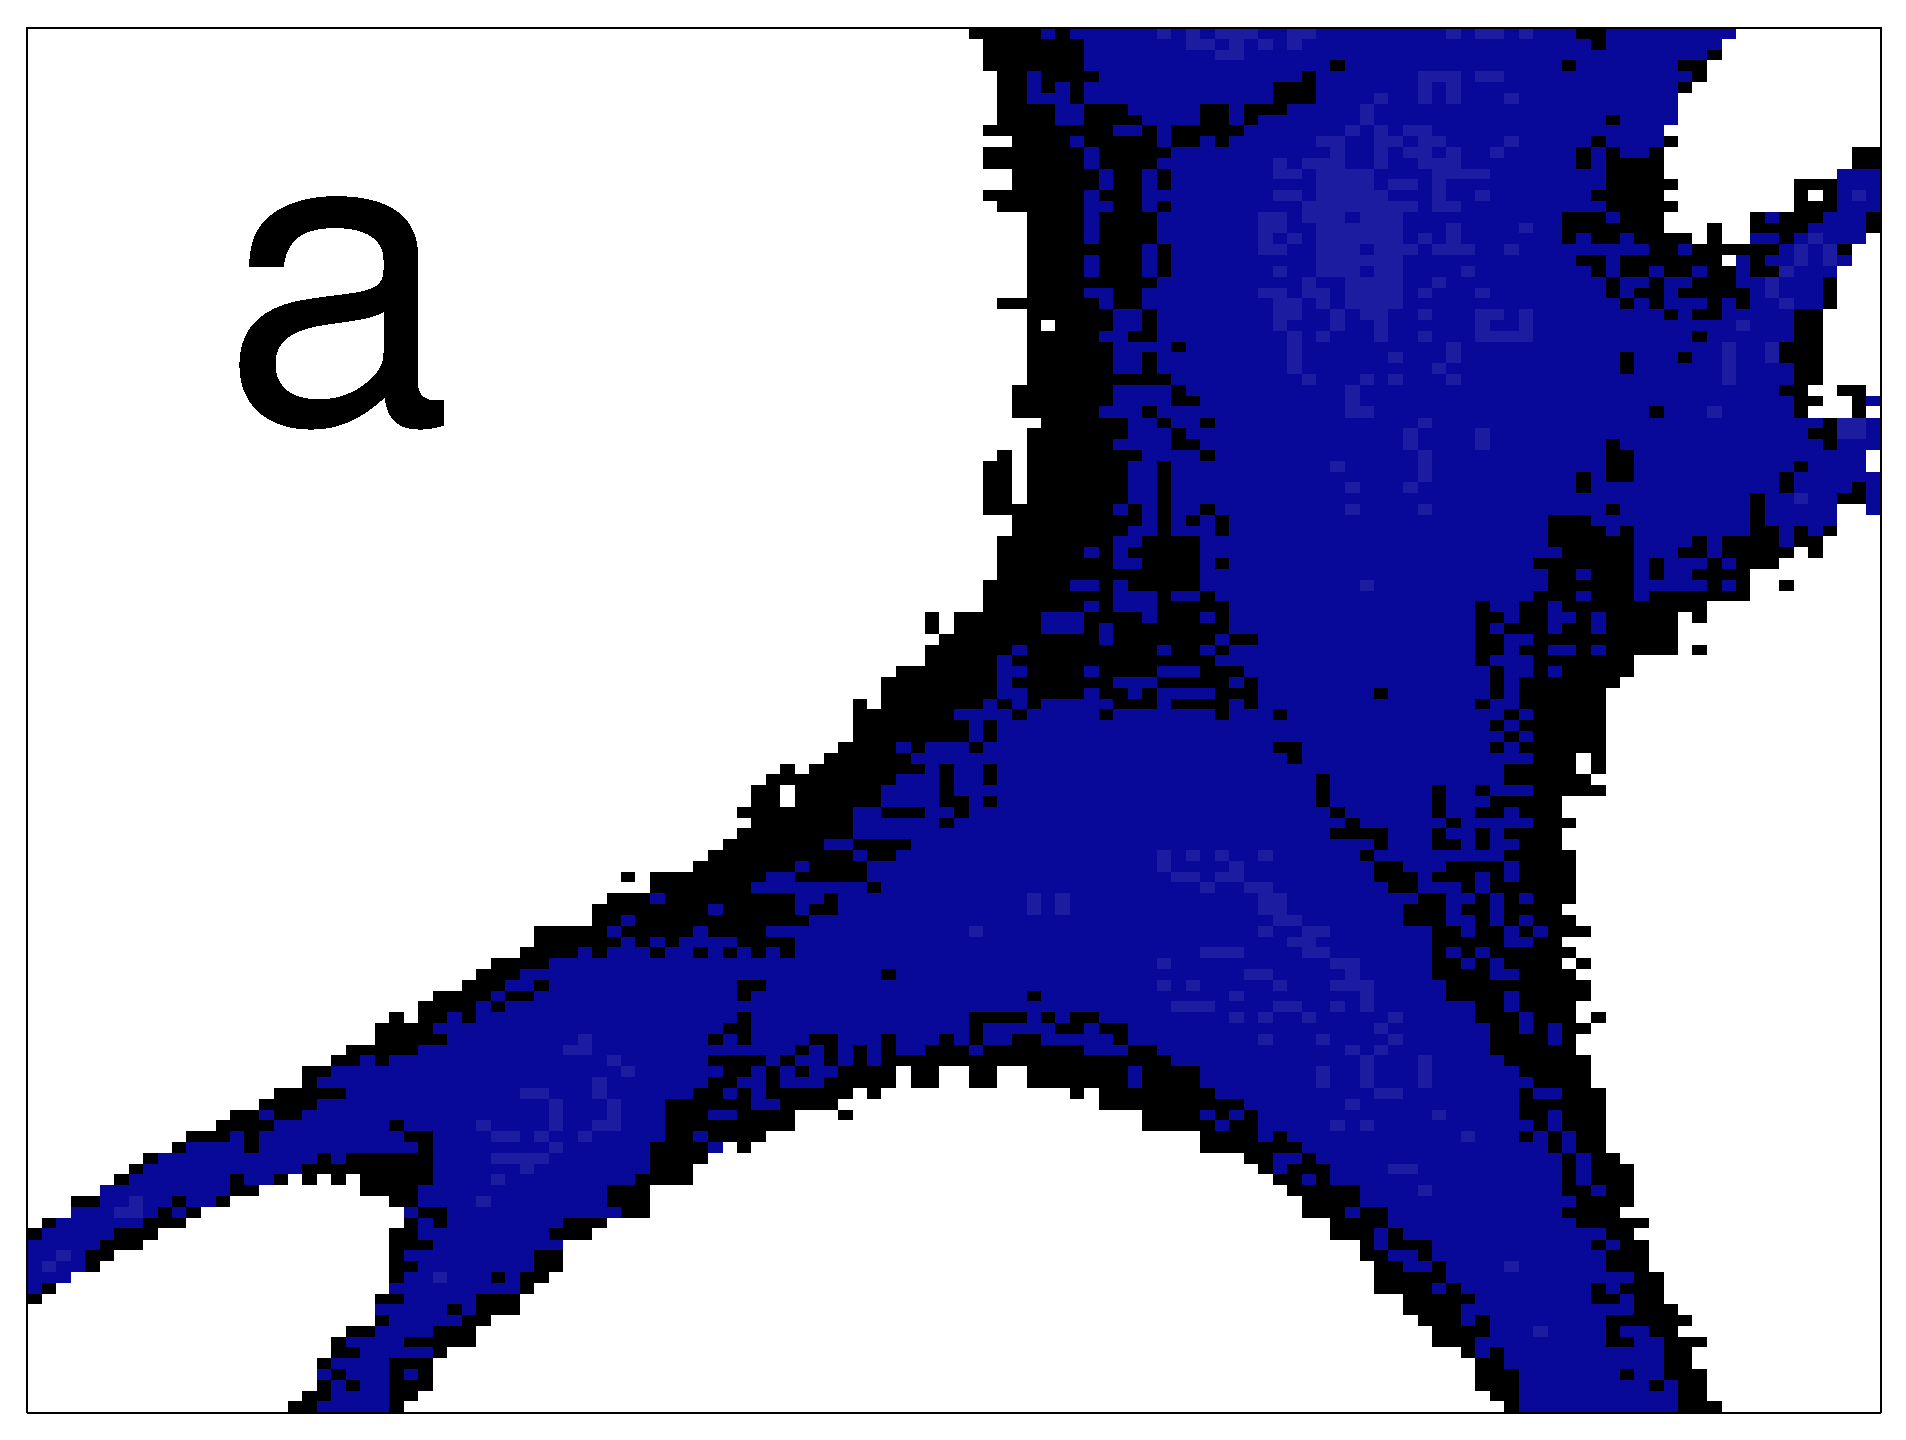
\includegraphics[width=0.3\textwidth]{m5}
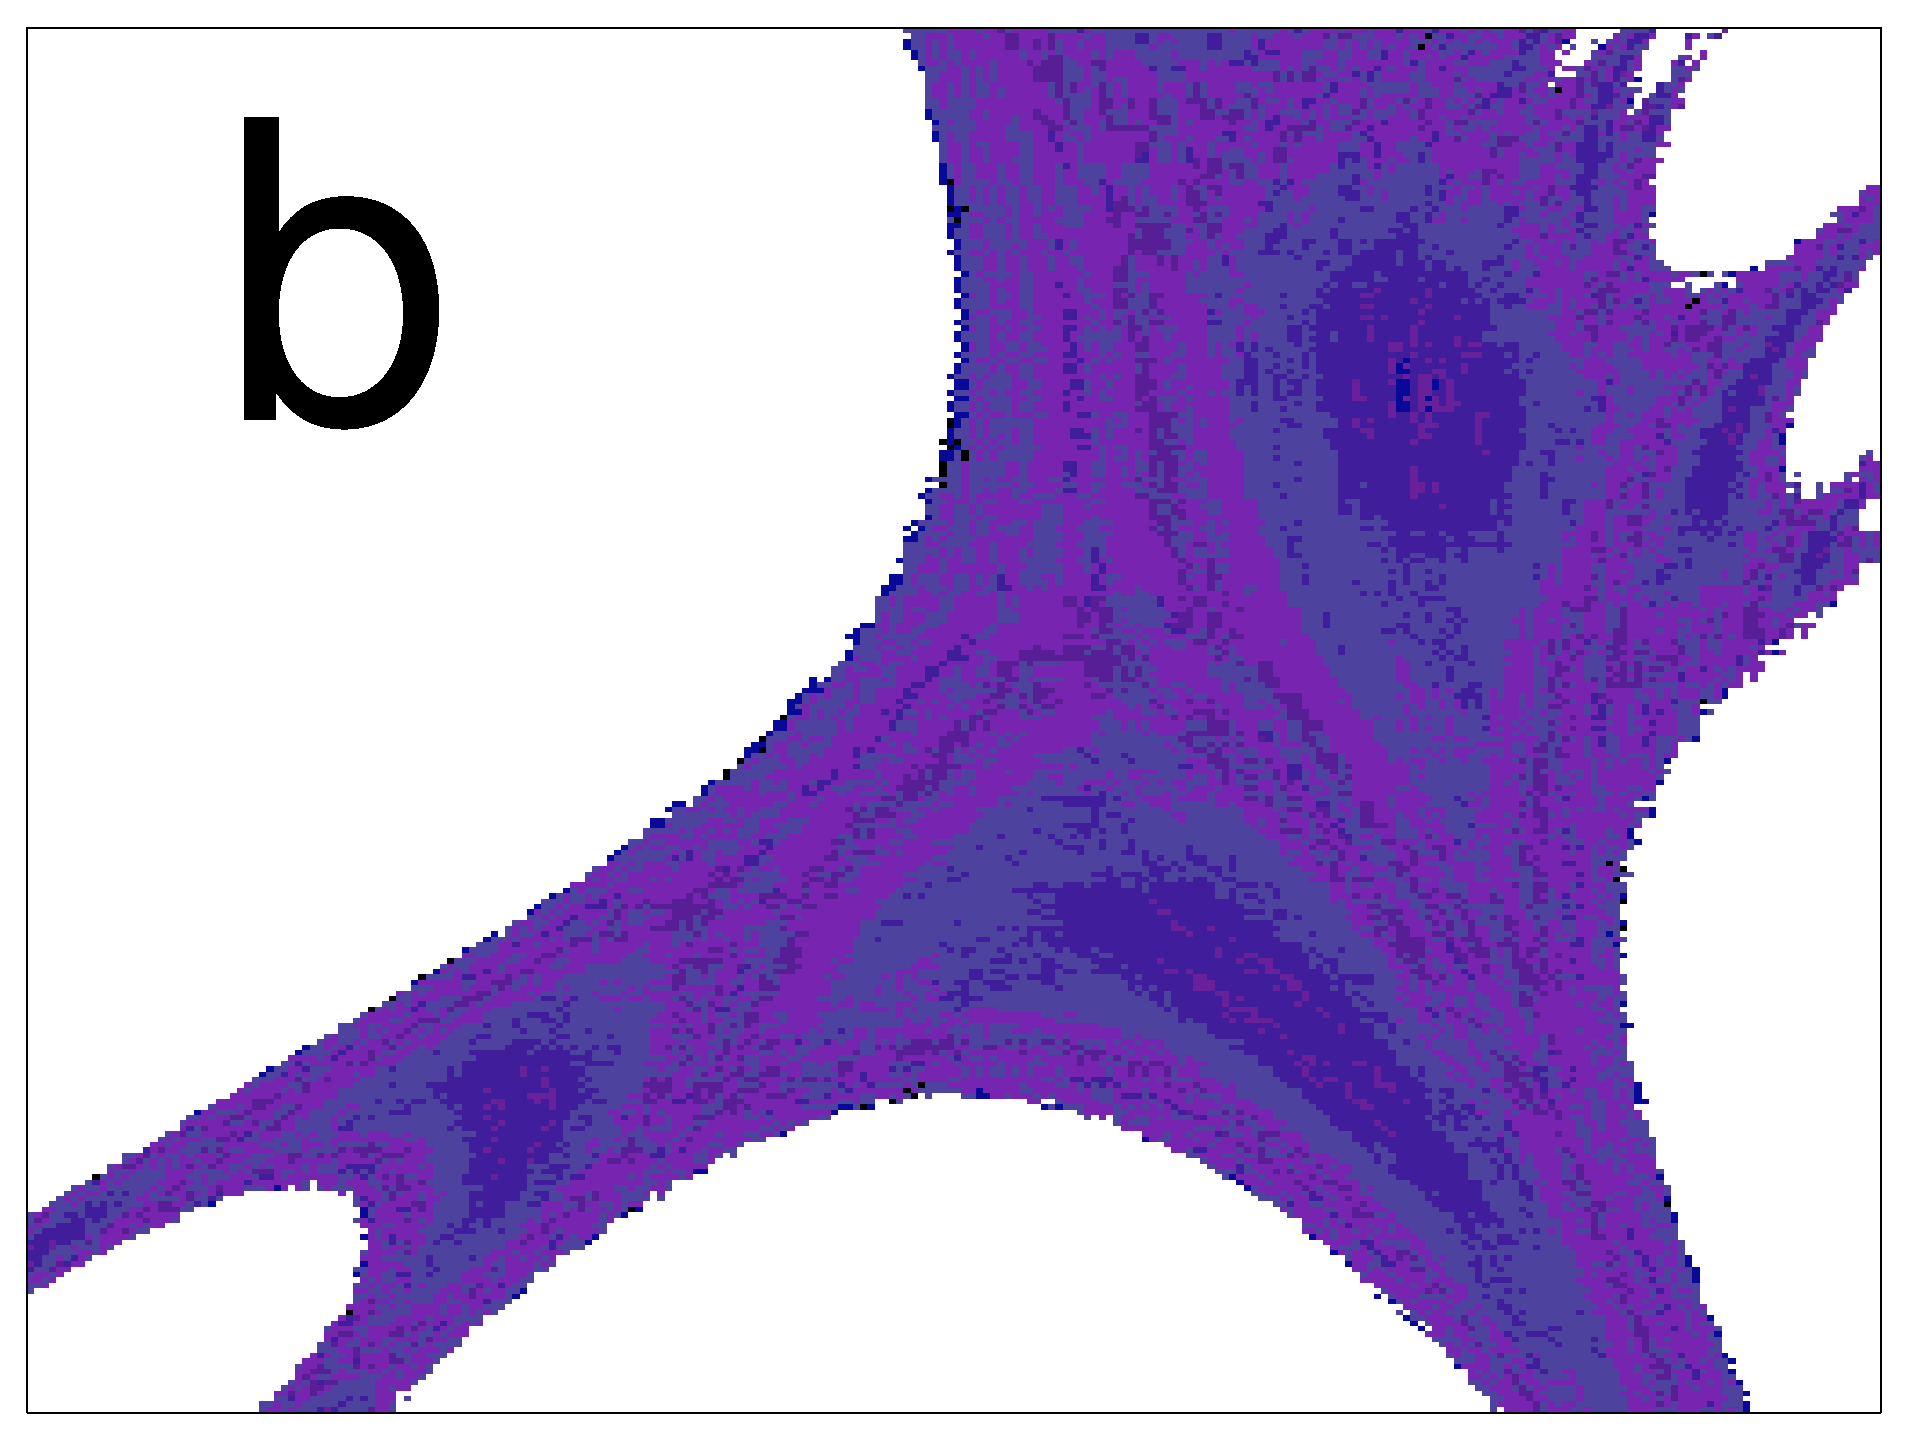
\includegraphics[width=0.3\textwidth]{m6}
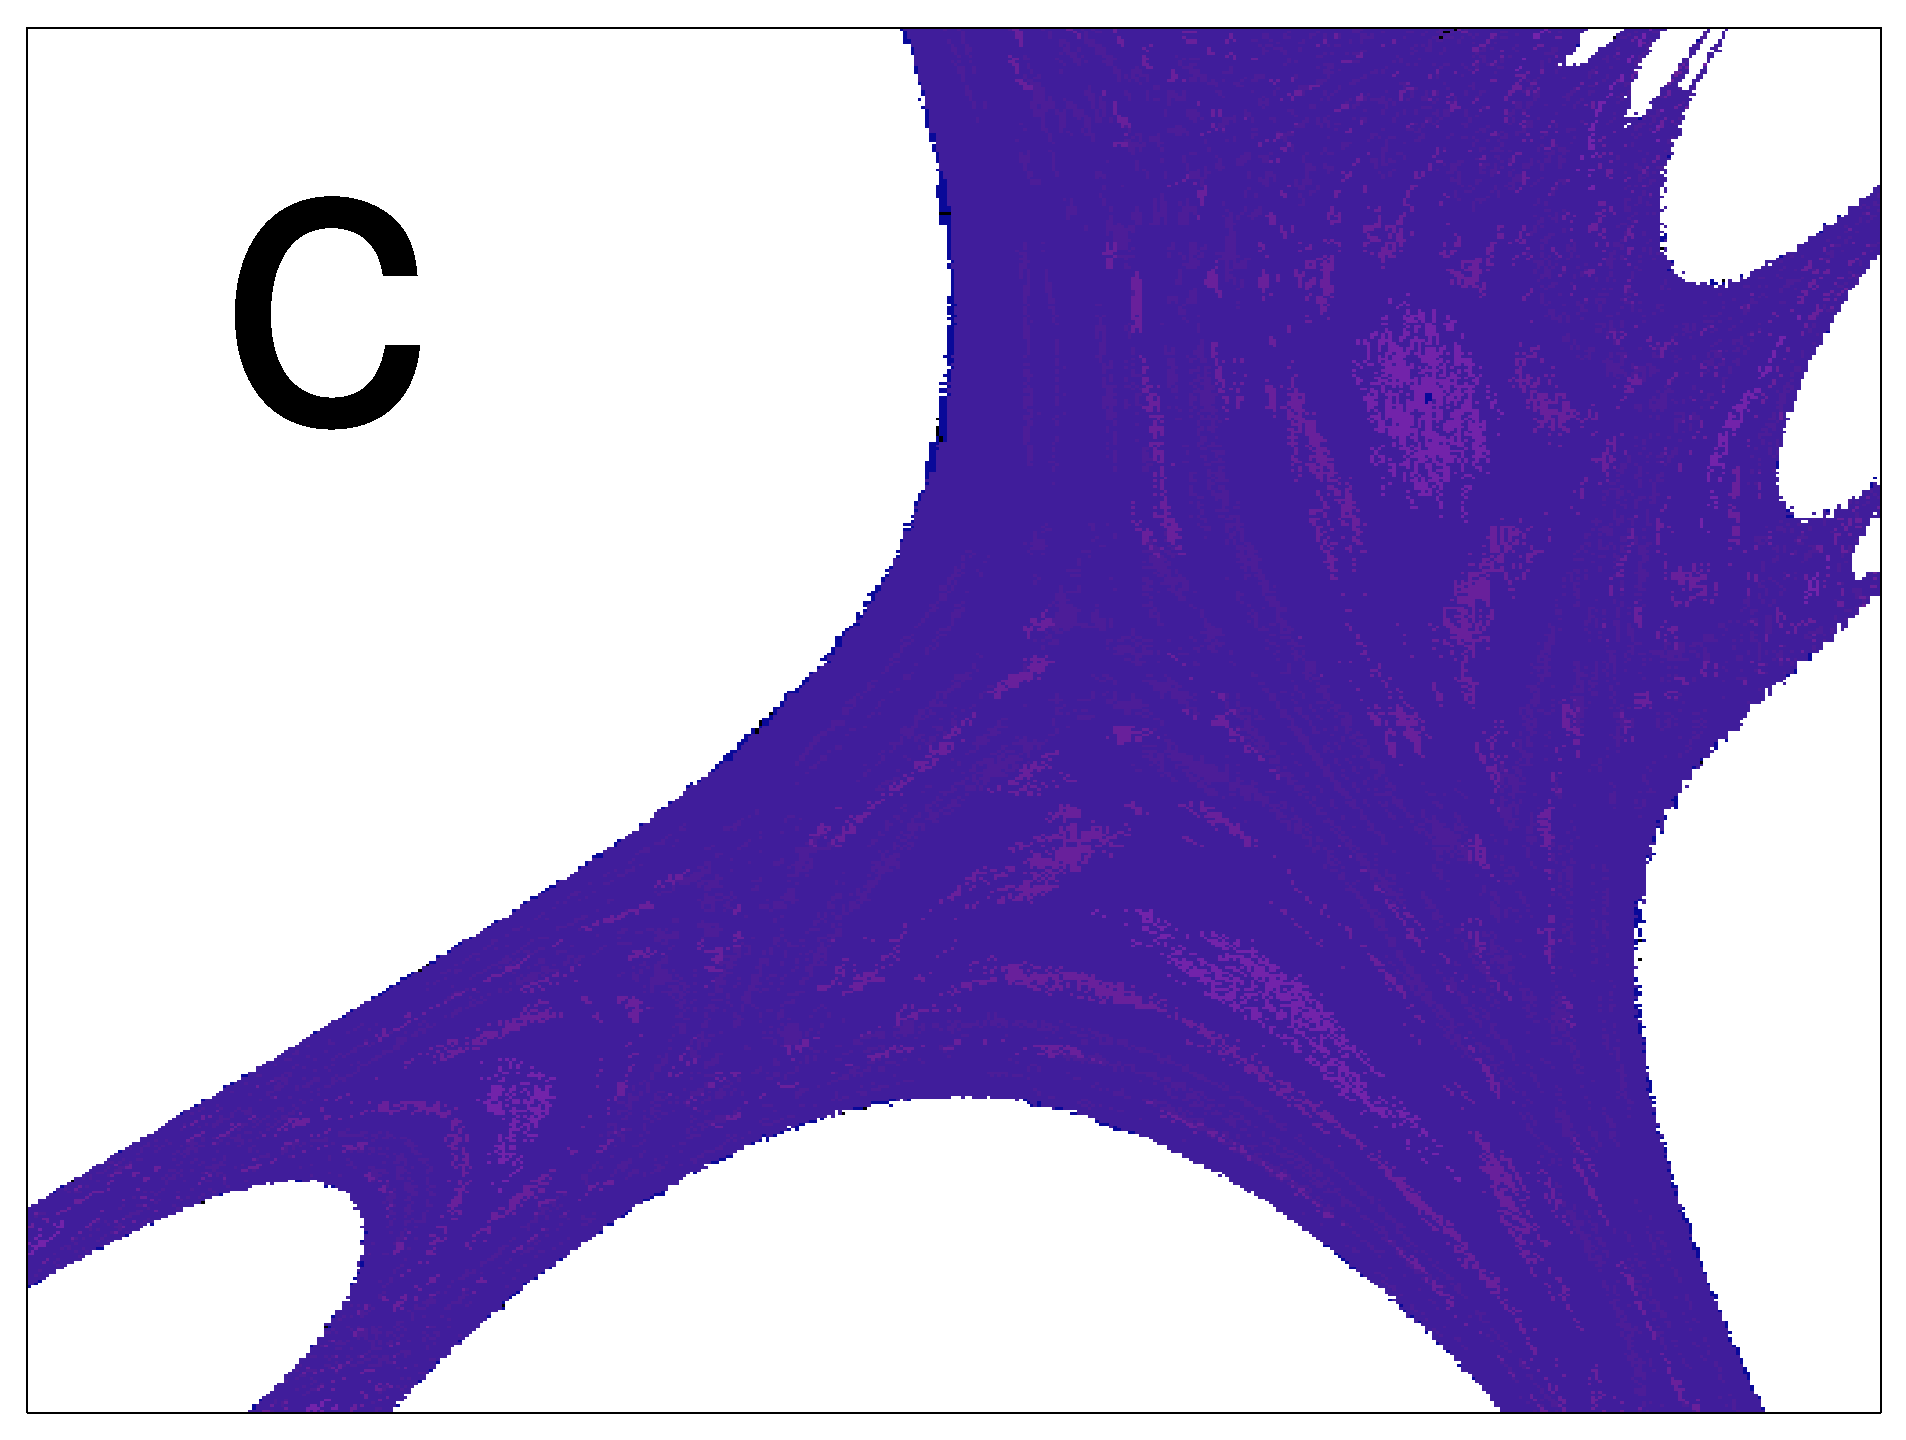
\includegraphics[width=0.3\textwidth]{m7}\\

\includegraphics[width=0.3\textwidth]{m8}
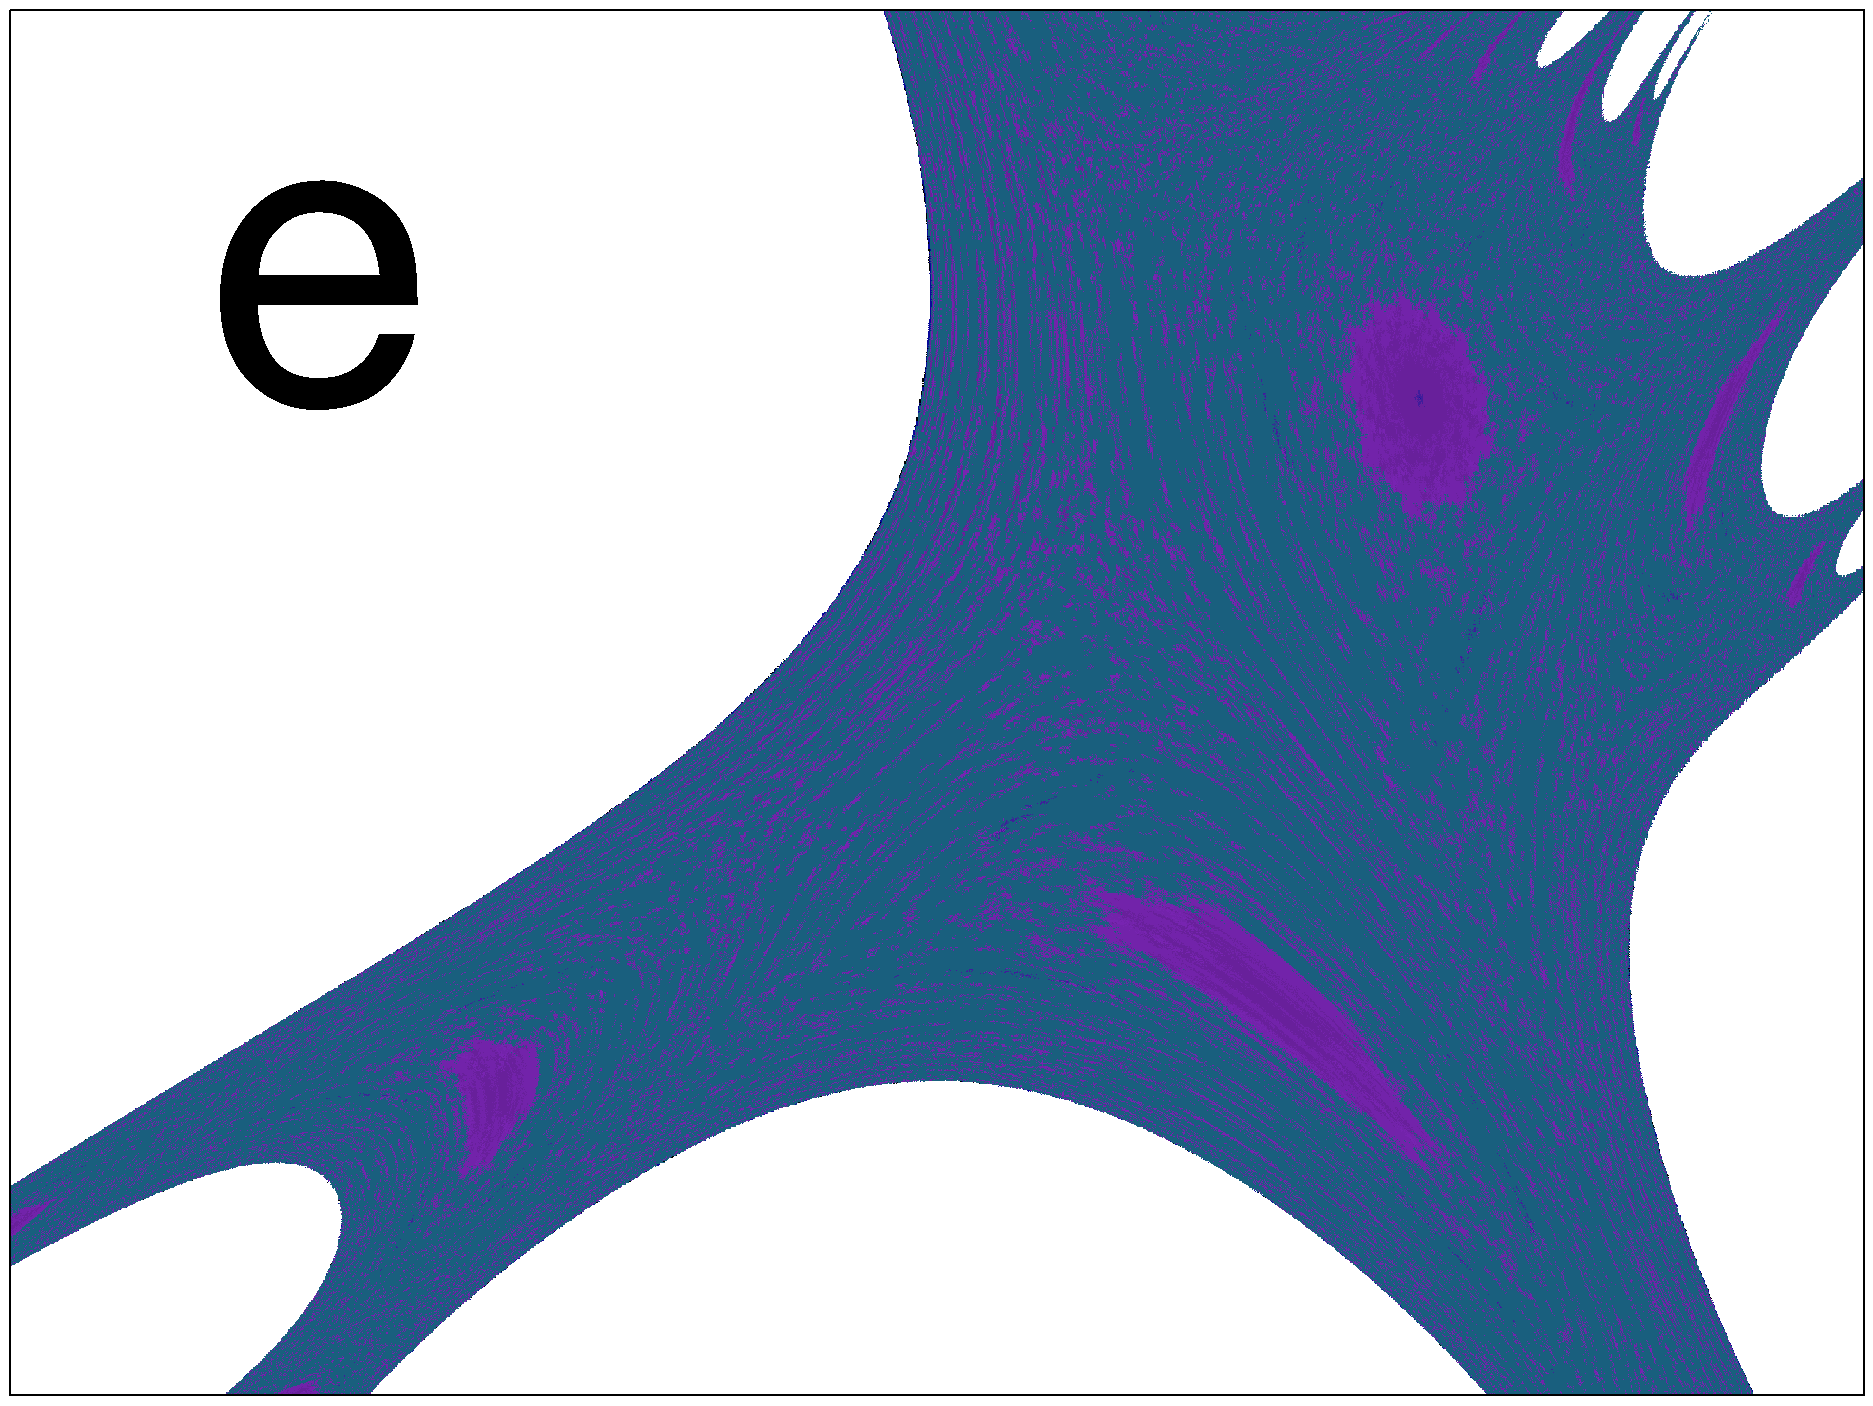
\includegraphics[width=0.3\textwidth]{m9}
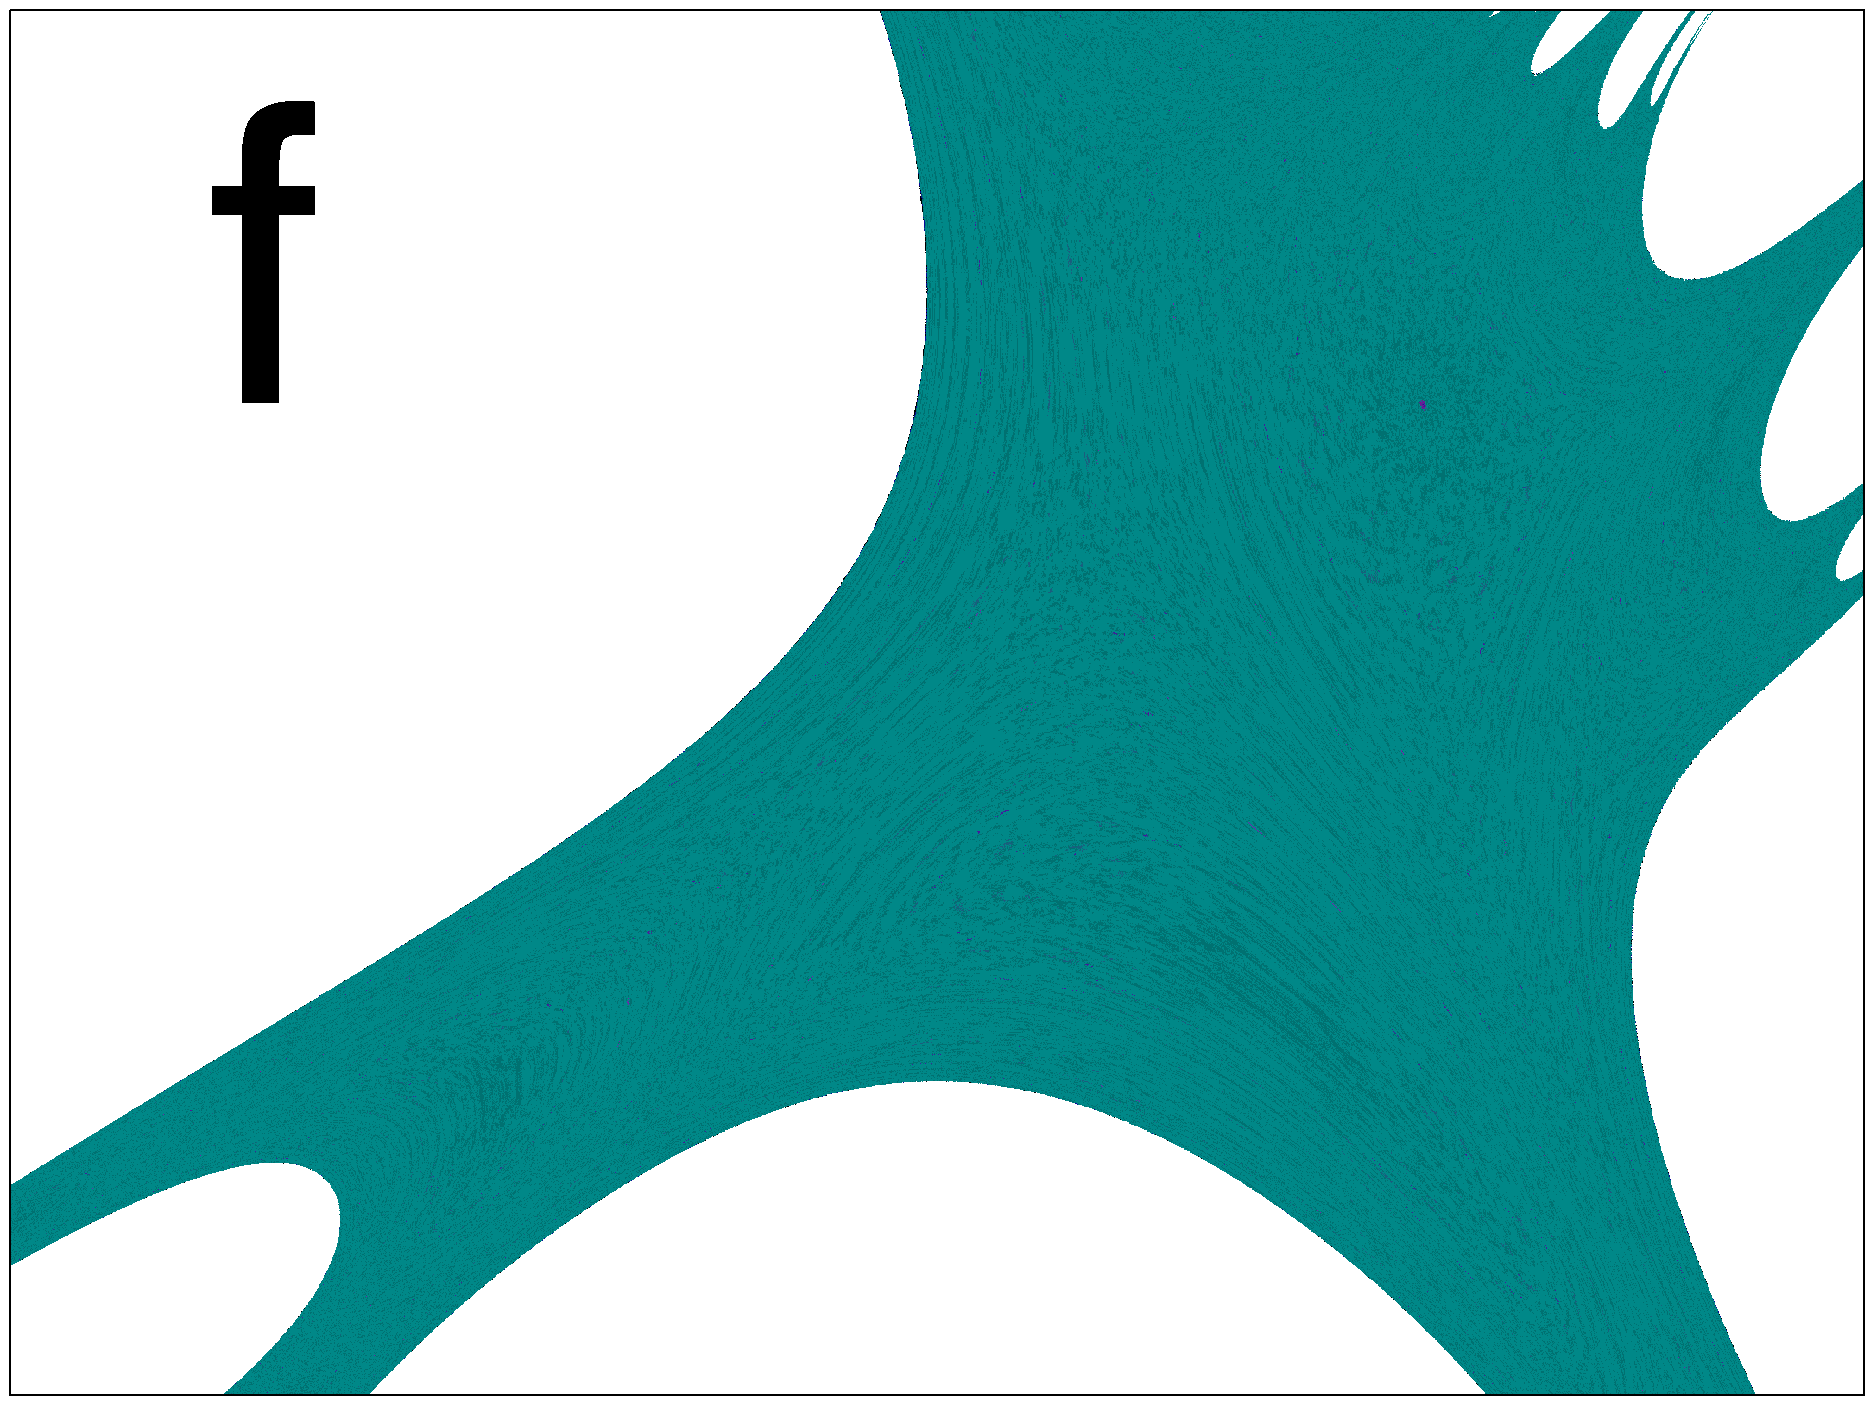
\includegraphics[width=0.3\textwidth]{m10}\\
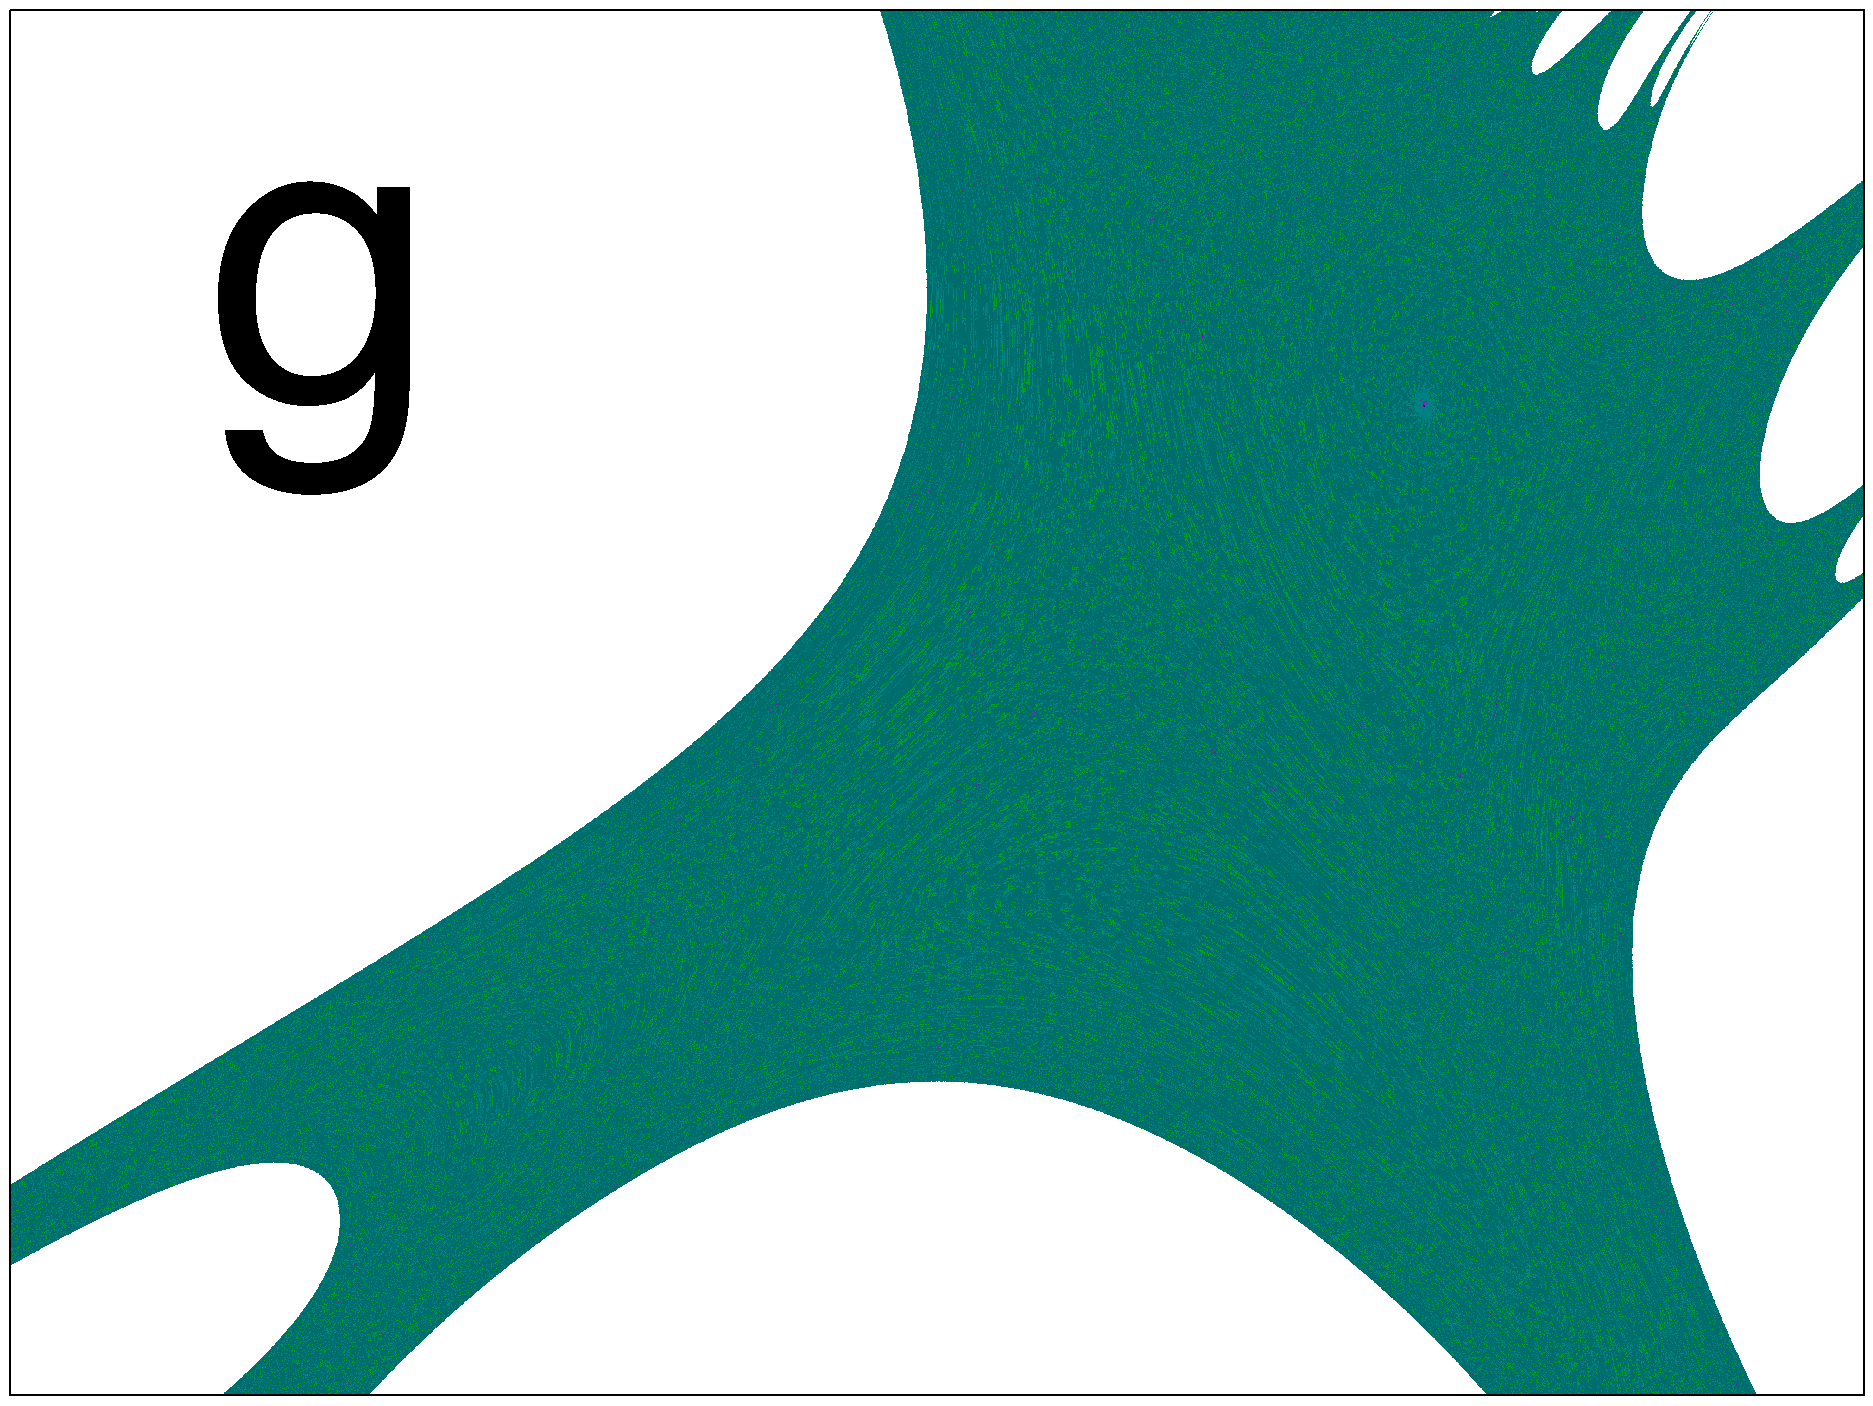
\includegraphics[width=0.3\textwidth]{m11}
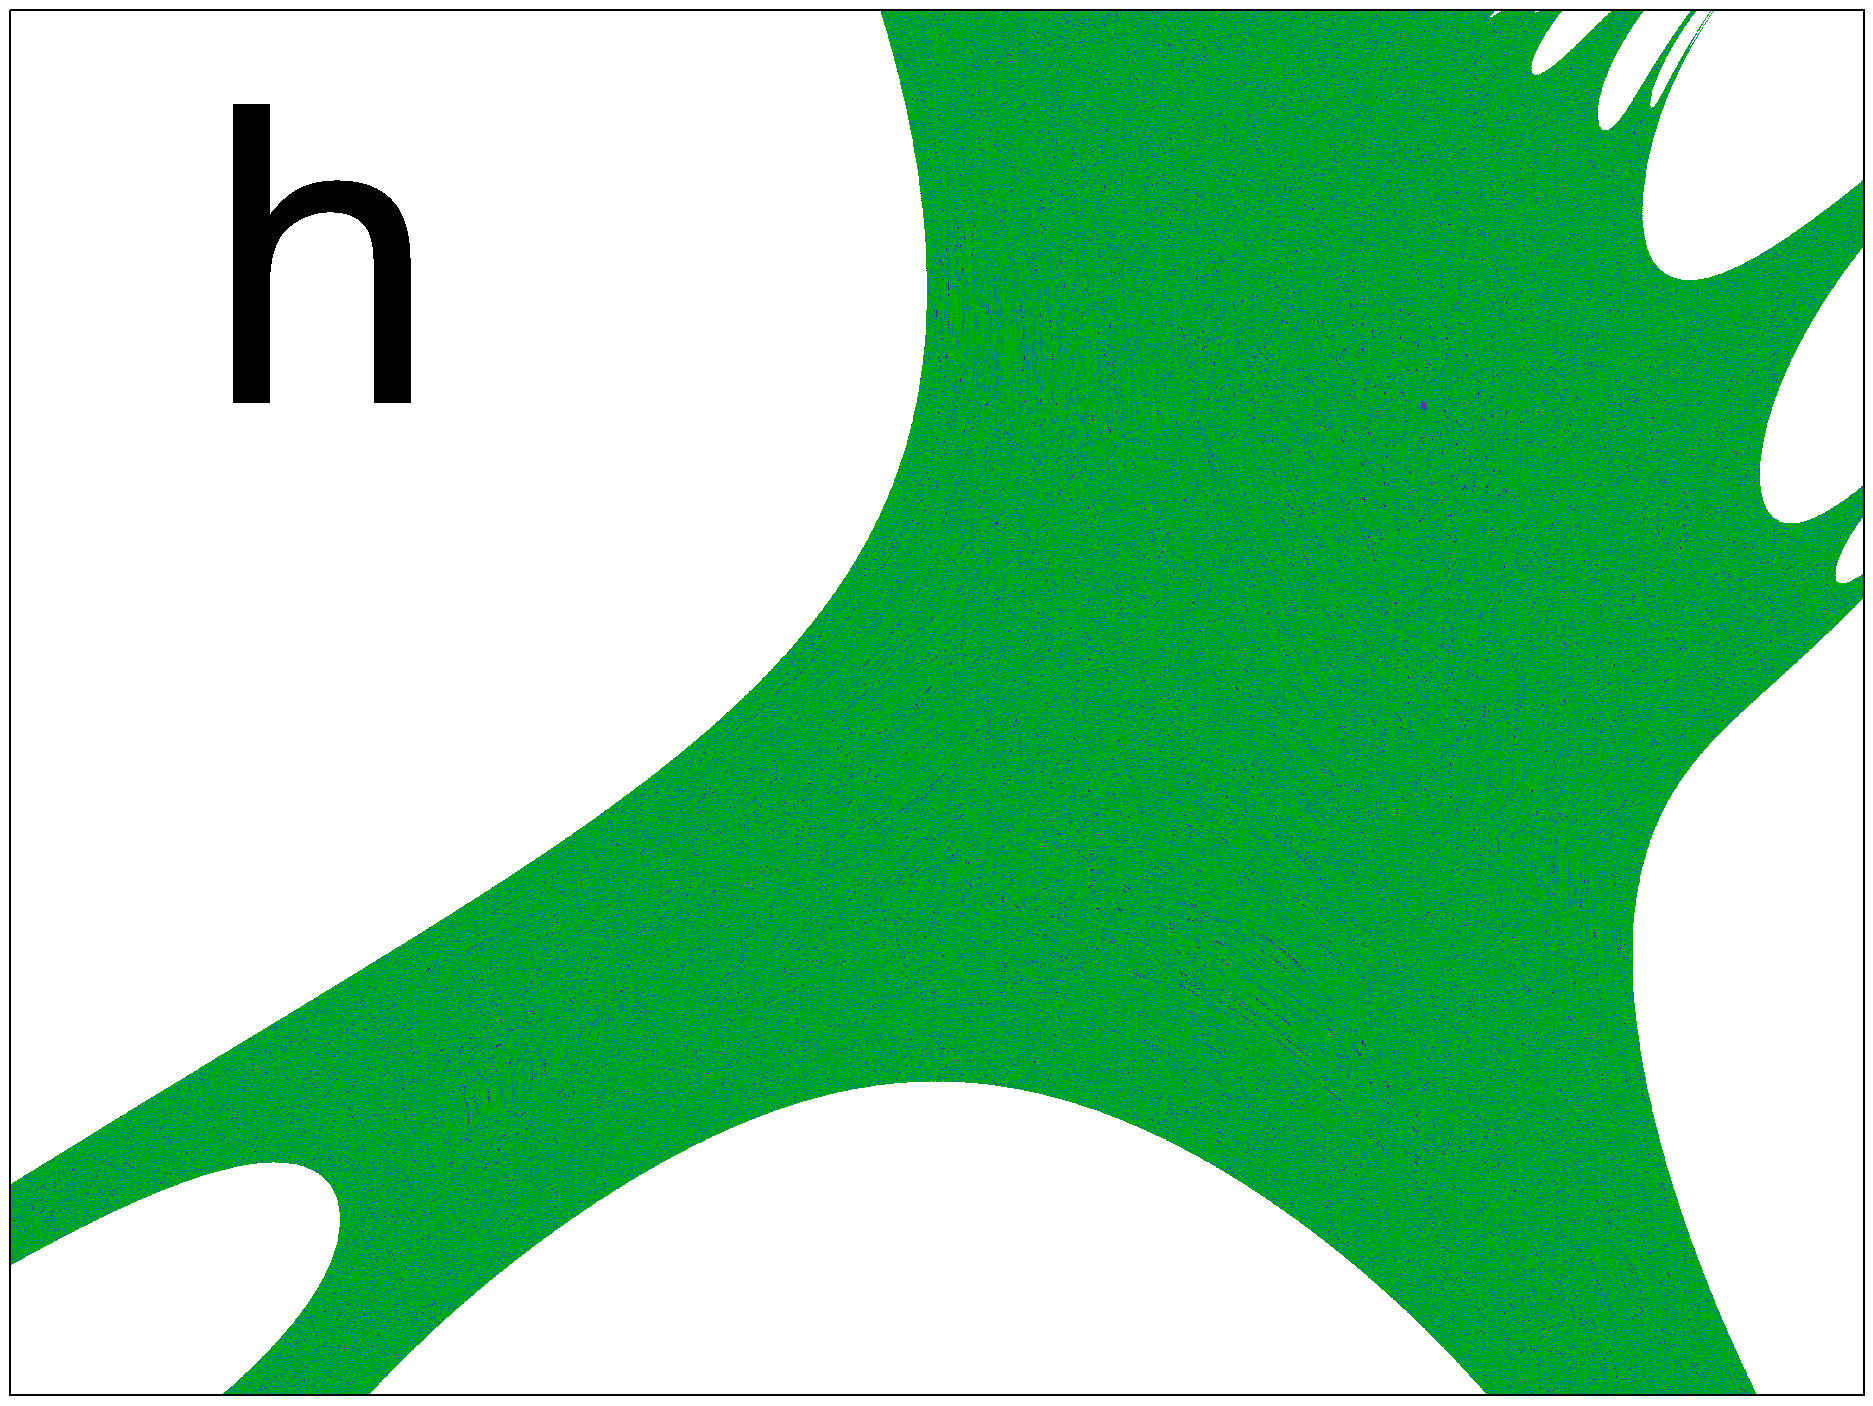
\includegraphics[width=0.3\textwidth]{m12}

\includegraphics[width=0.3\textwidth]{m13}\\

\includegraphics[width=0.3\textwidth]{m14}
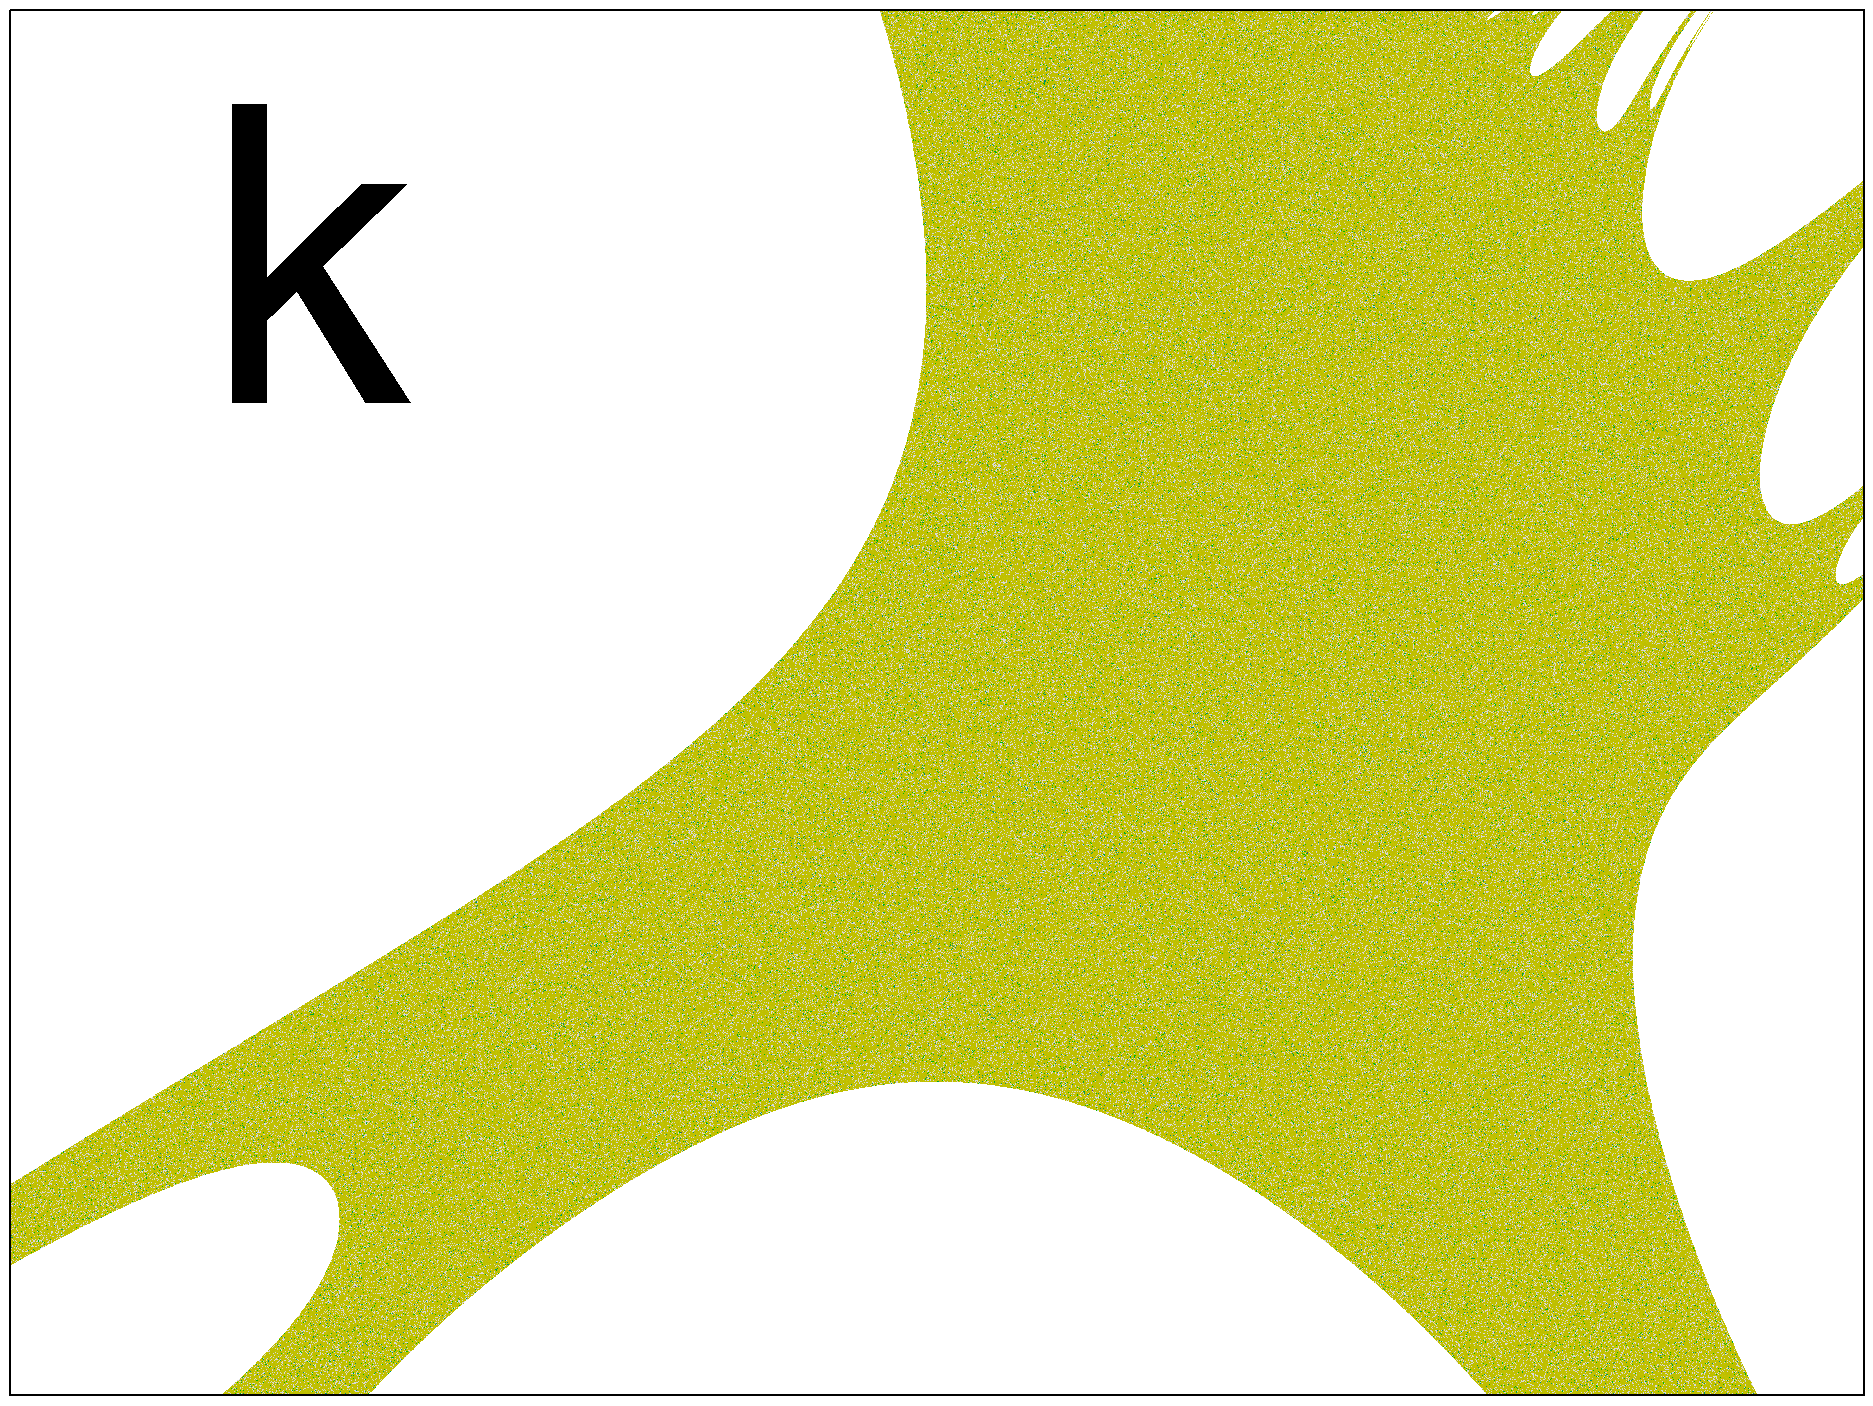
\includegraphics[width=0.3\textwidth]{m17}
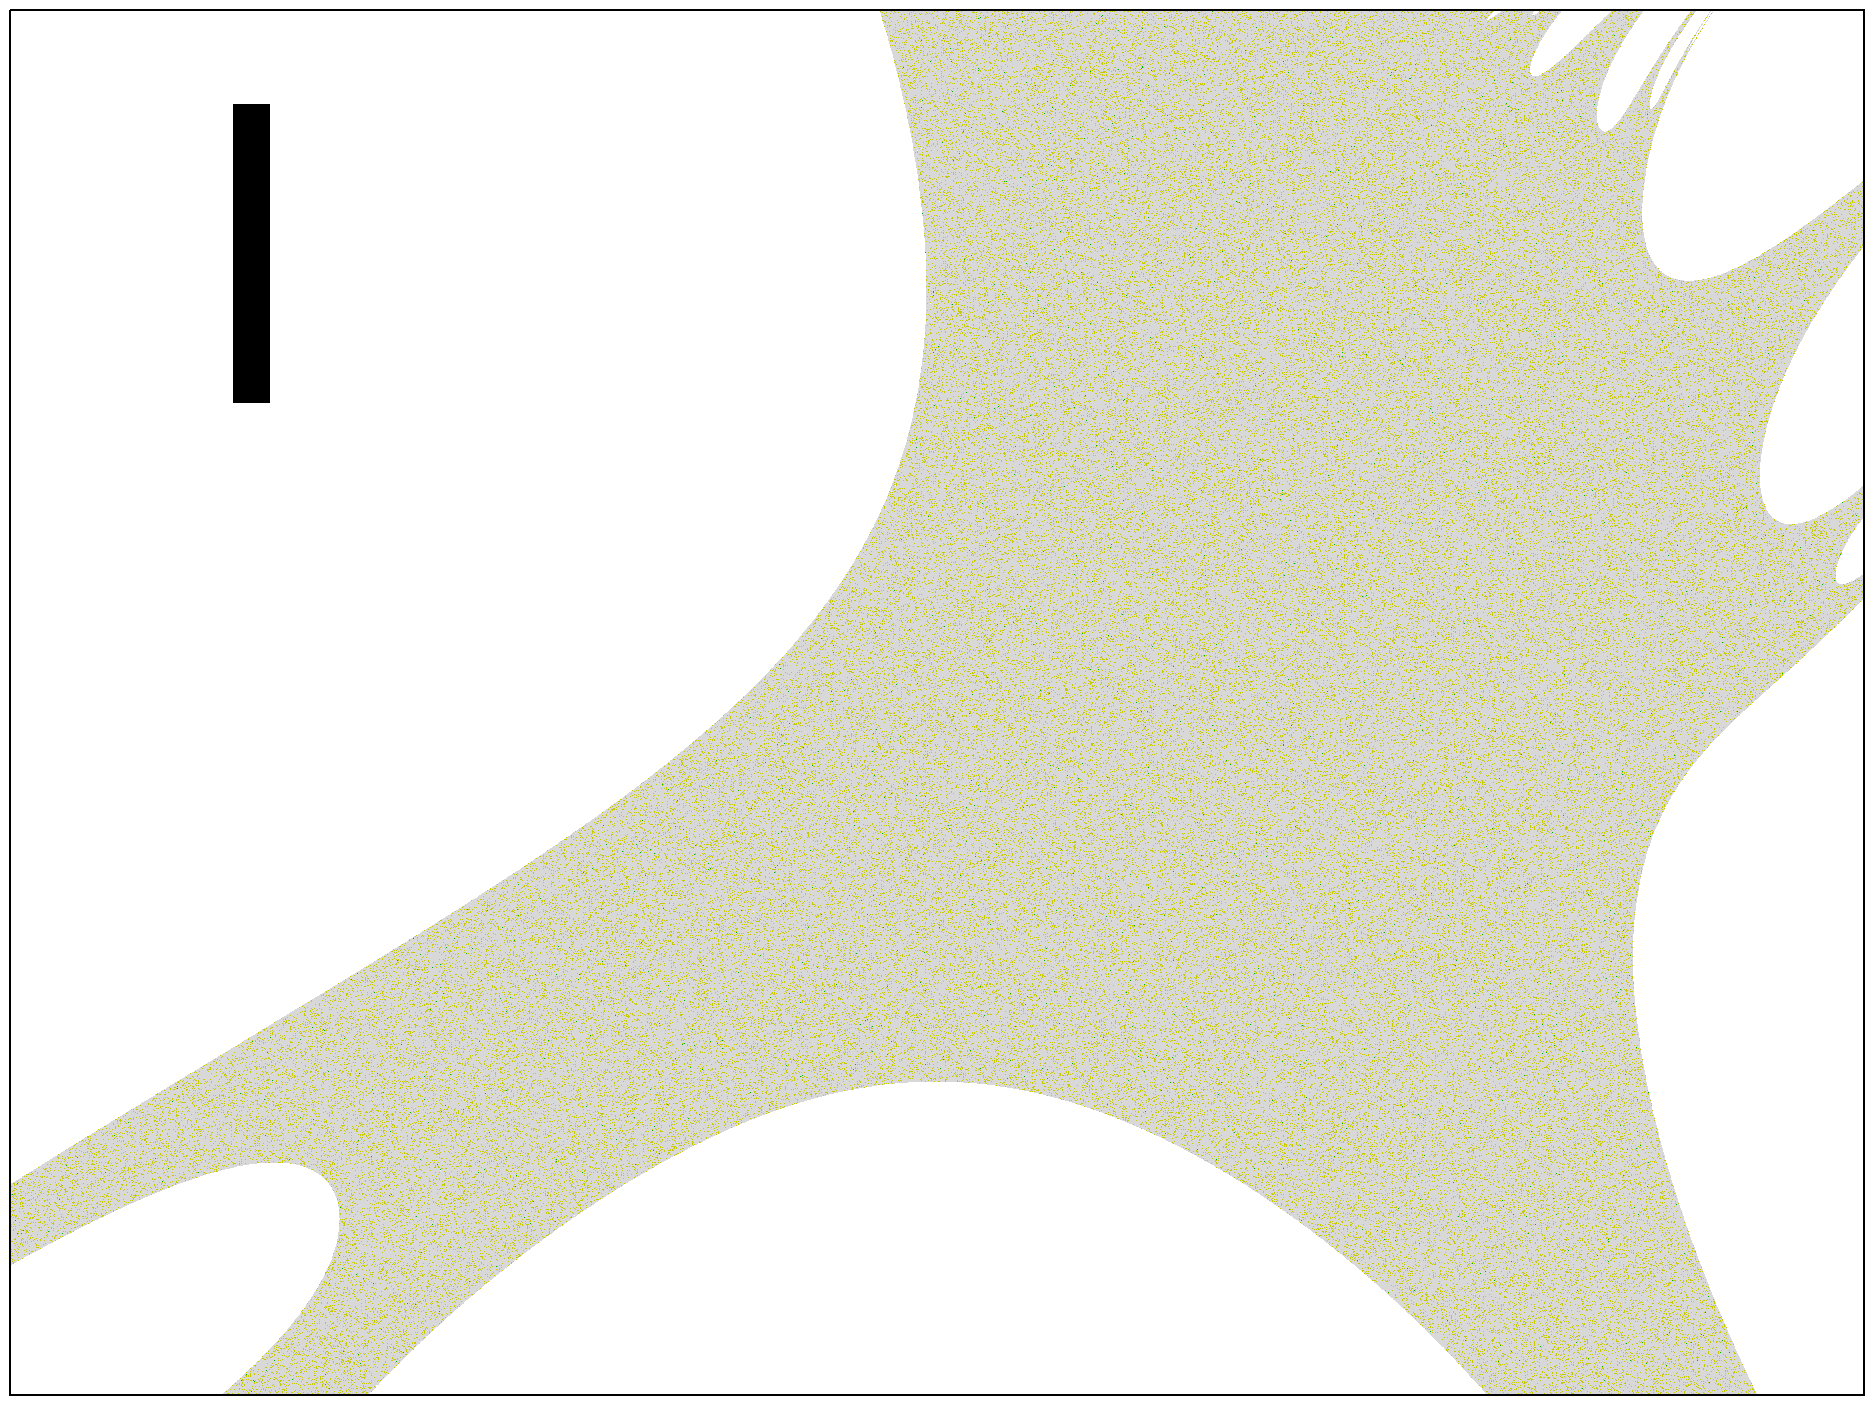
\includegraphics[width=0.3\textwidth]{m18}\\
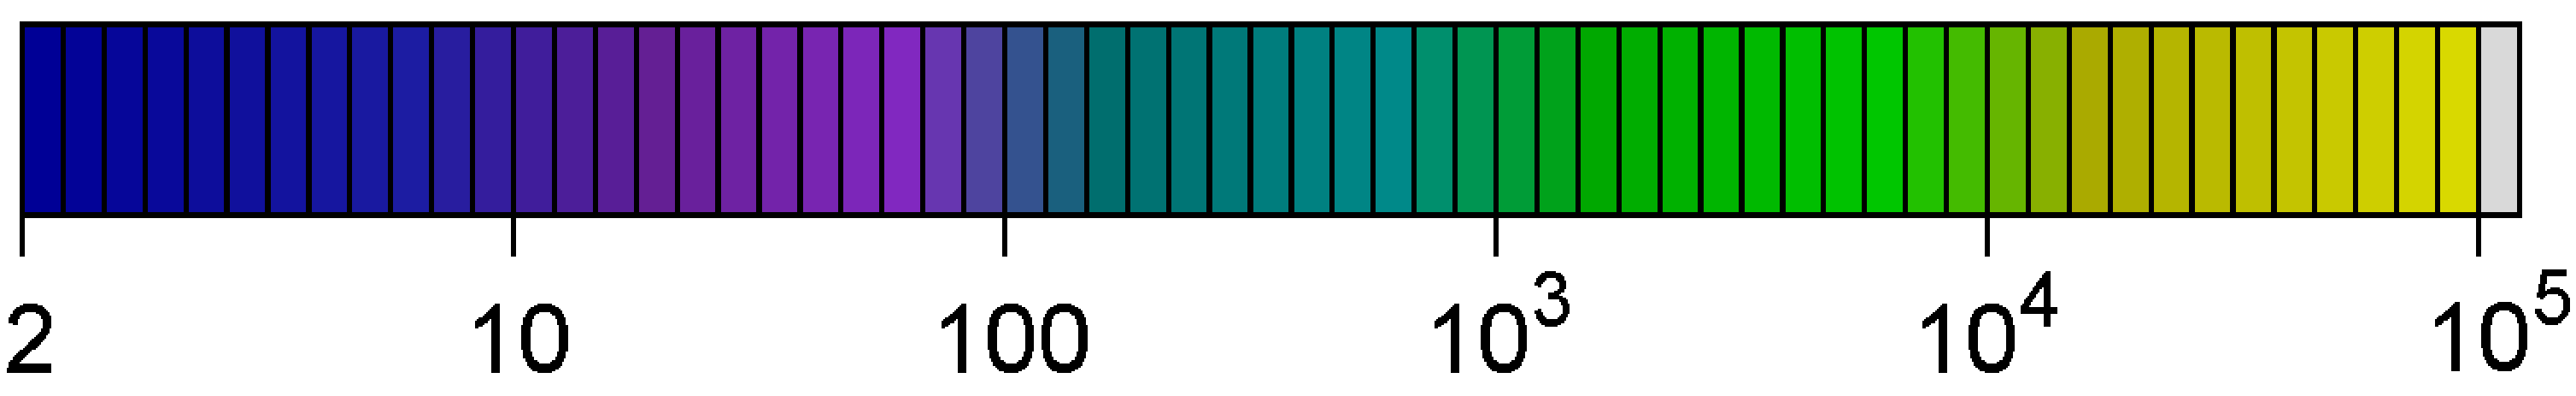
\includegraphics[width=1\textwidth]{ColorMapConEje}
\end{tabular}
\caption{Domains of attraction xxxxx for: a) $n_b=5$, (b) $n_b=6$, c) $n_b=7$, d) $n_b=8$, e) $n_b=9$, f) $n_b=10$, g) $n_b=11$, h) $n_b=12$, i) $n_b=13$, j) $n_b=14$, k) $n_b=17$, l) $n_b=18$. Coefficients $a_0$ to $a_{11}$ have the values $\{a_i\}=\{-1.0, 0.9, 0.4, -0.2, -0.6, -0.5, 0.4, 0.7, 0.3, -0.5, 0.7,-0.8\}$. 
The initial conditions $\{x_0,y_0\}$  are  in the square  $x_0\in[-2,+2]$, $y_0\in[-2,+2]$, on a grid with step $0.001$. Each initial condition is iterated $10^5$ times. }.
\label{fig:avvel}
\end{figure}. 
%=====================================================
%==================================================
\begin{figure}
    \centering
    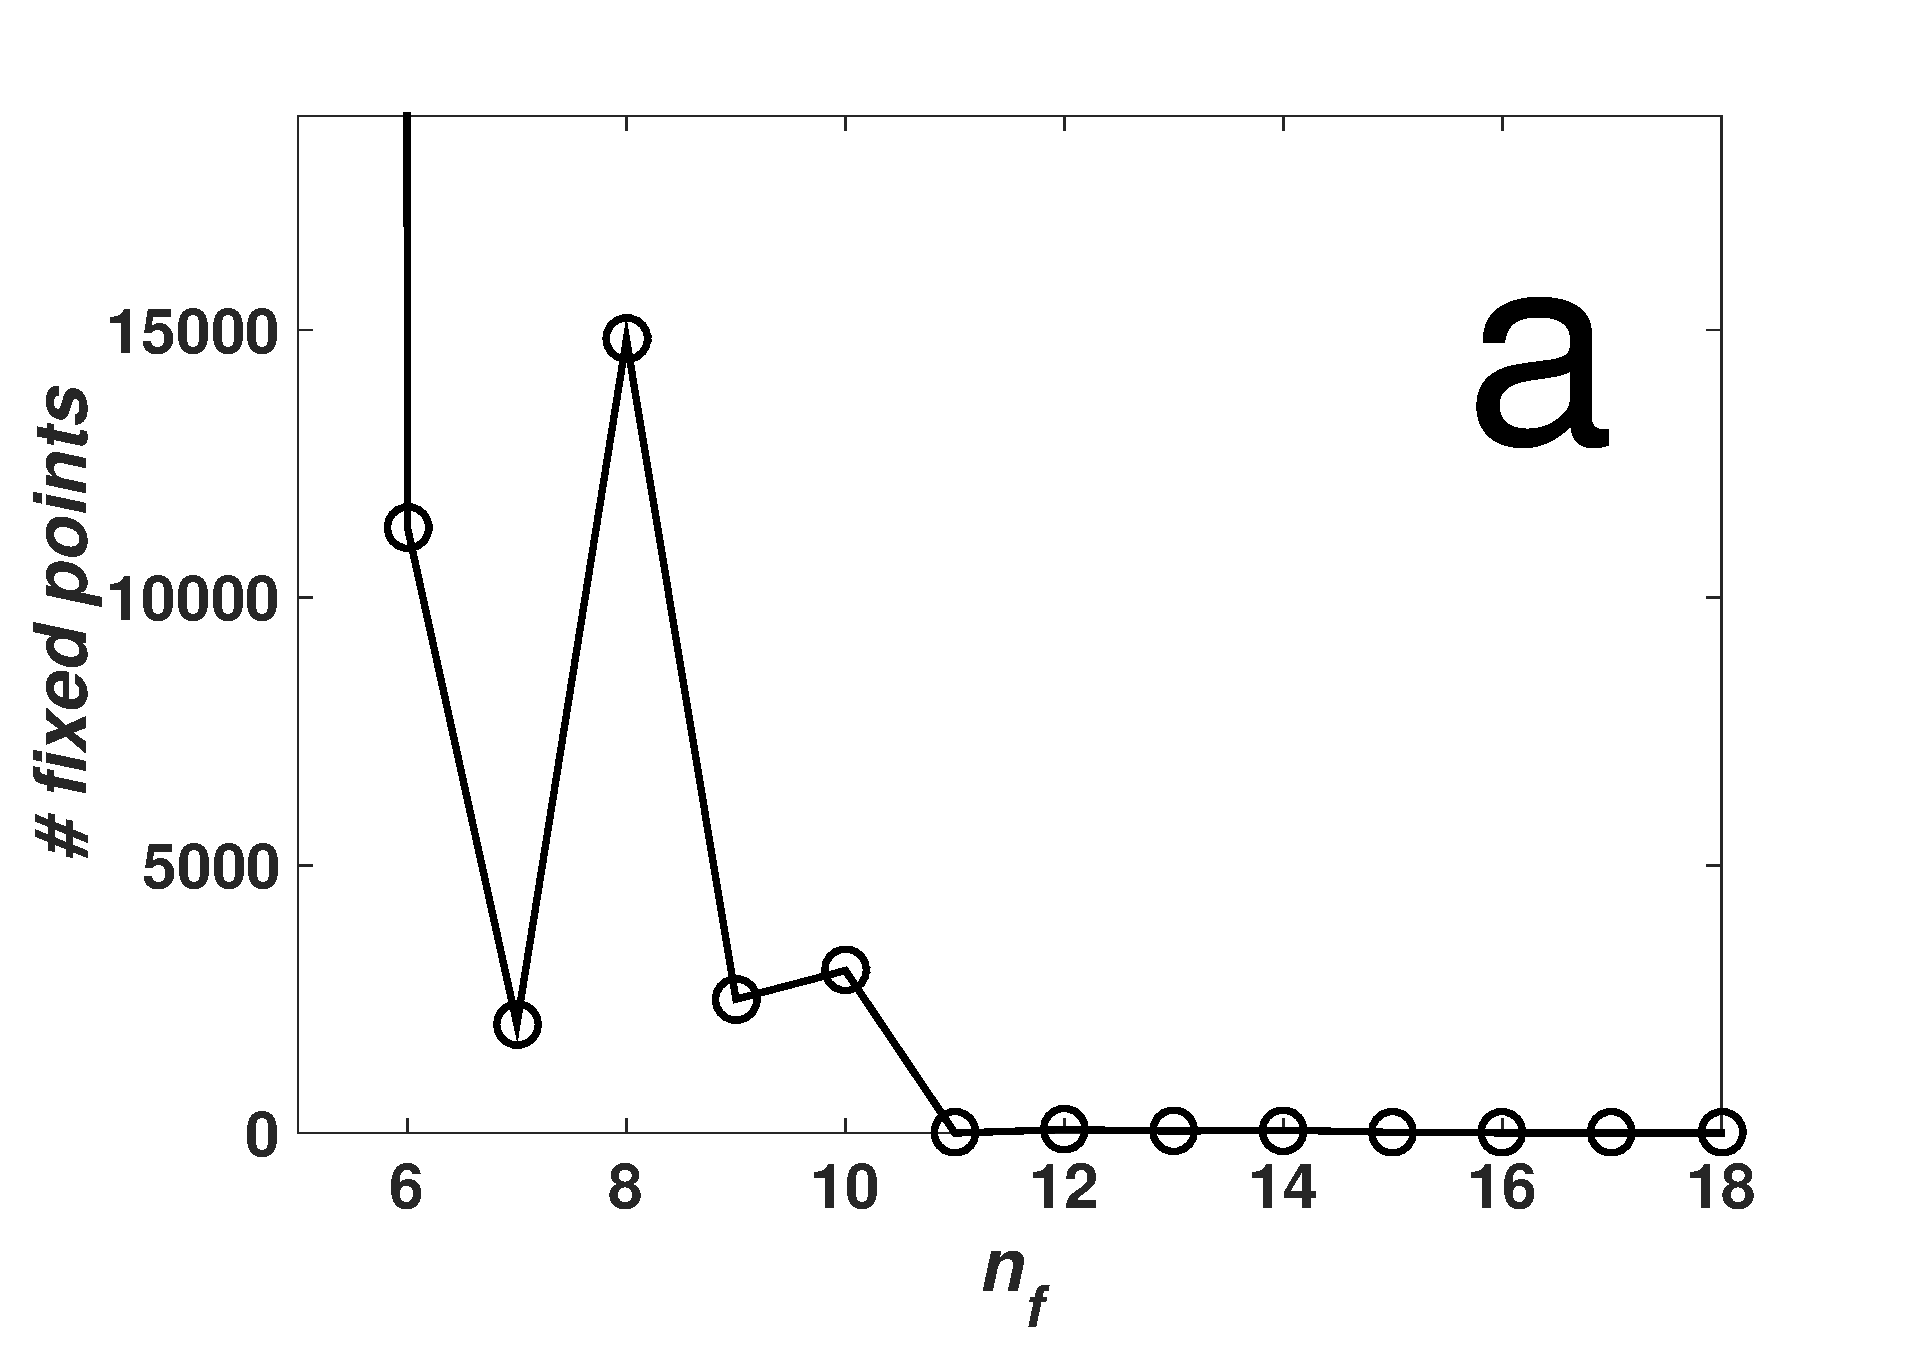
\includegraphics[width=0.7\columnwidth]{ptosfijos}\\
    \caption{Quantity of fixed points.}
    \label{fig:puntosfijos}

\end{figure}
%==================================================
%==================================================
\begin{figure}
    \centering
    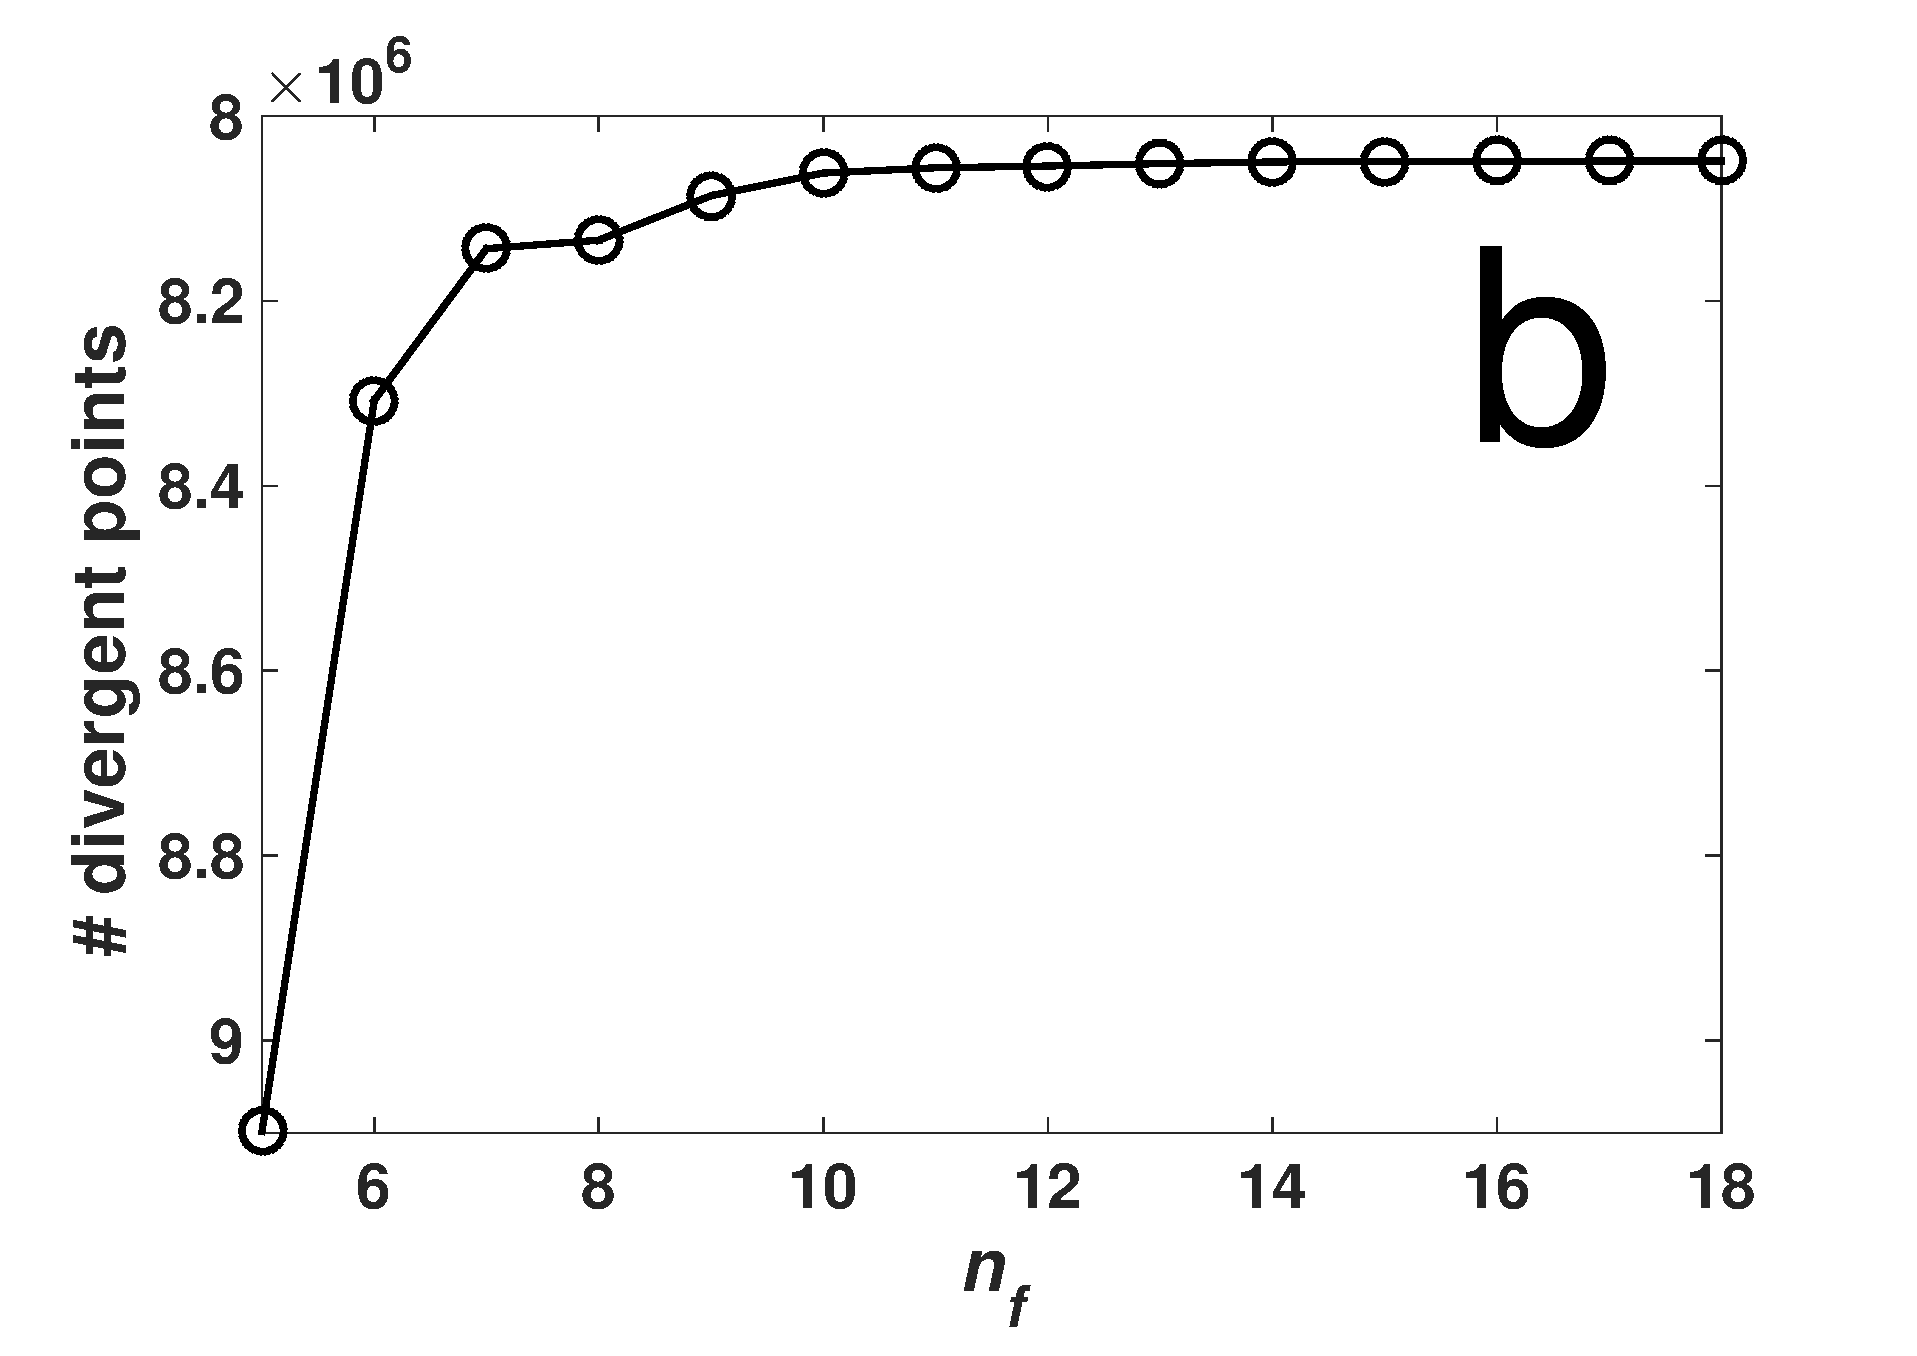
\includegraphics[width=0.7\columnwidth]{divergen}\\
    \caption{Quantity of divergent points.}\label{fig:puntosdivergentes}

\end{figure}
%==================================================
%==================================================
\begin{figure}
    \centering
        \includegraphics[width=0.7\columnwidth]{periodosmaximos}\\
    \caption{Maximum periods reached.}\label{fig:periodosmaximos}

\end{figure}
%==================================================
%==================================================
\begin{figure}
    \centering
        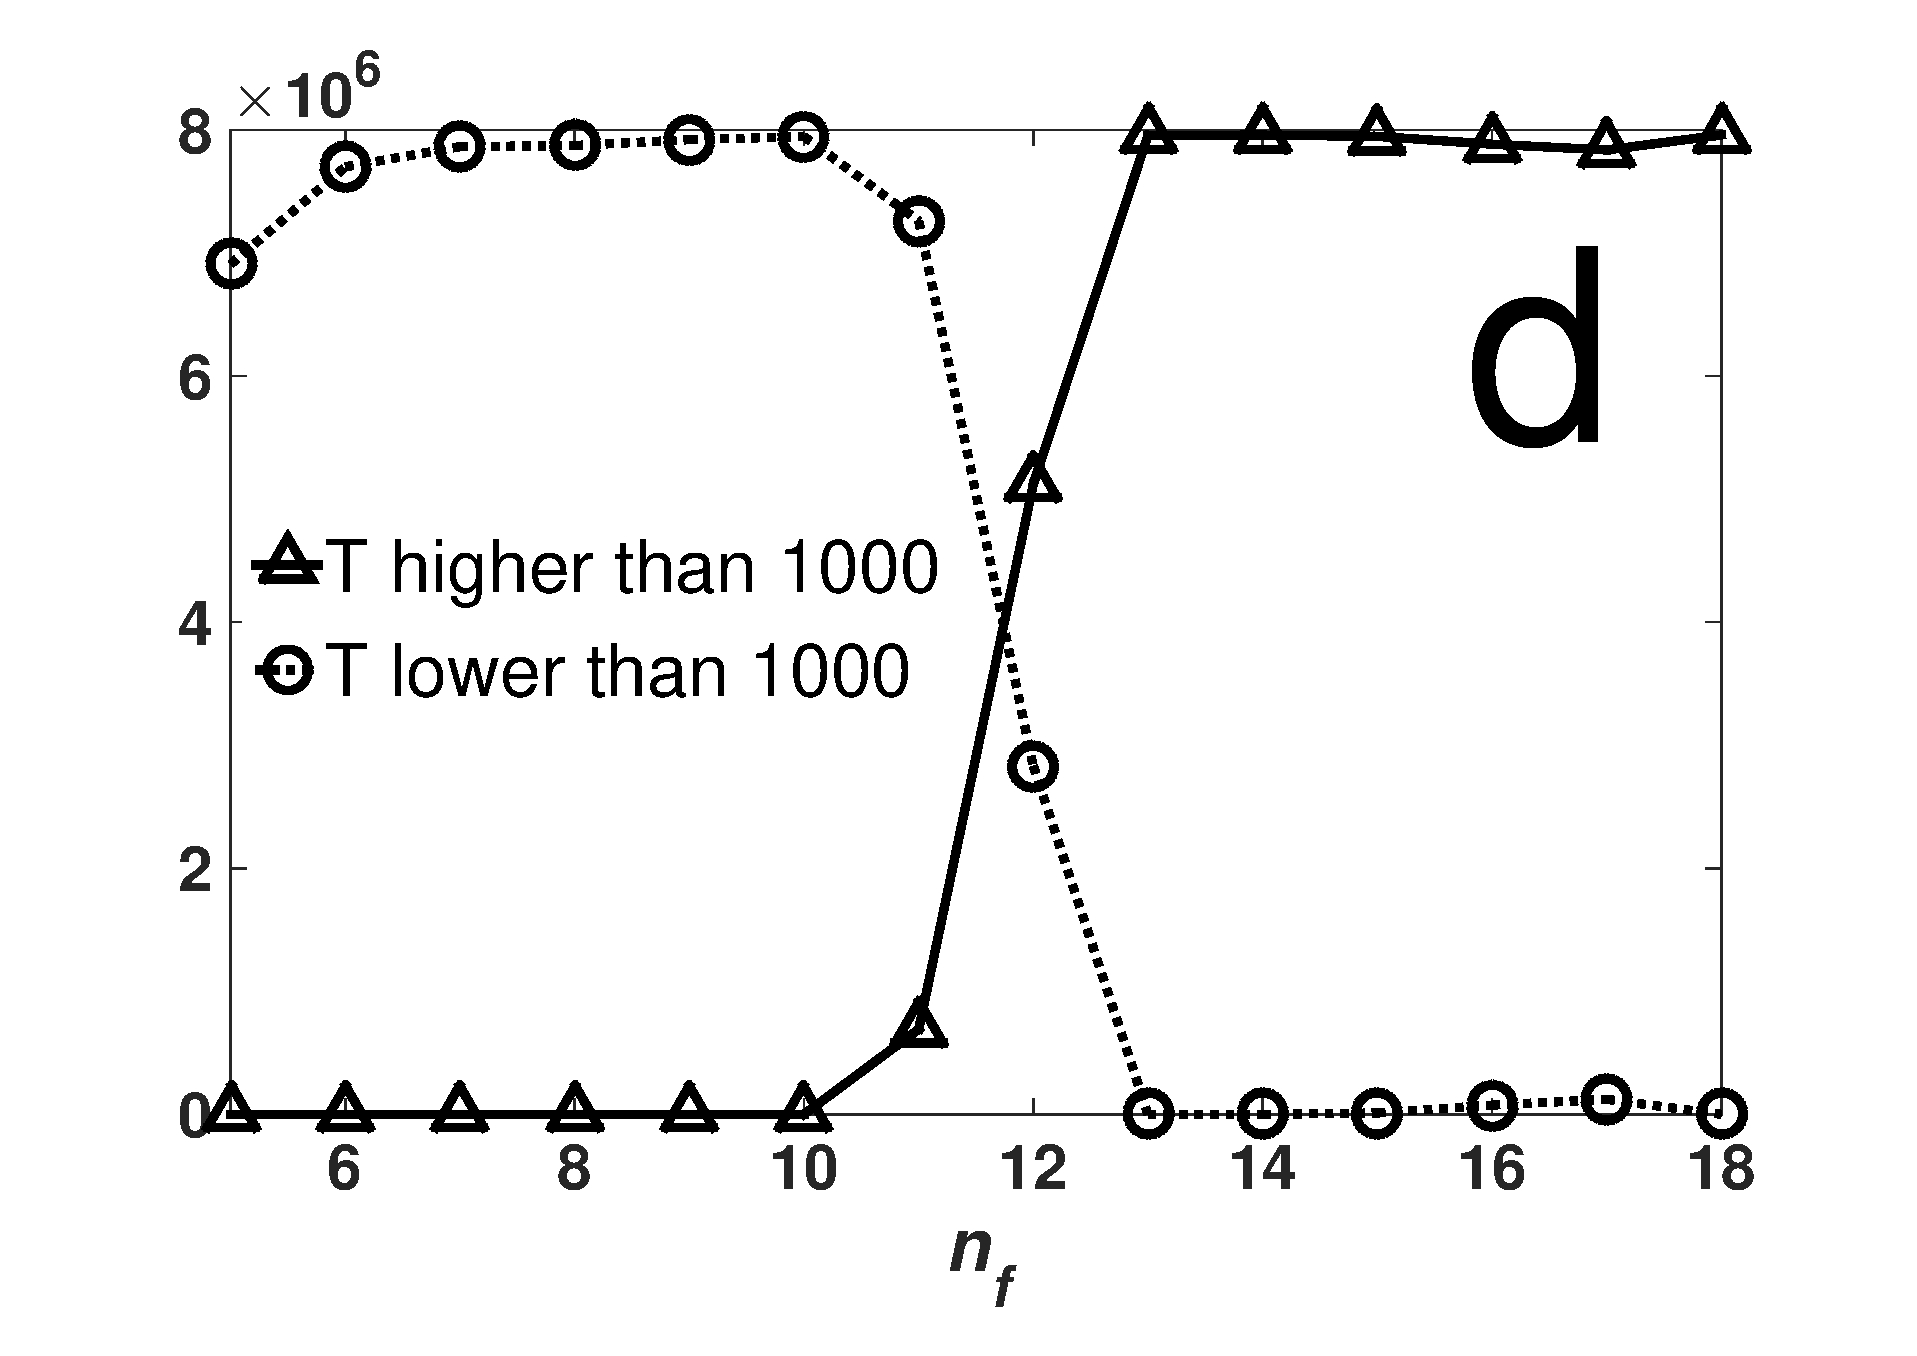
\includegraphics[width=0.9\columnwidth]{Puntos}\\
    \caption{Quantity of initial conditions with period ($T$) higher and lower than $1000$.}\label{fig:puntos}

\end{figure}
%==================================================
%==================================================
\begin{figure}
    \centering
        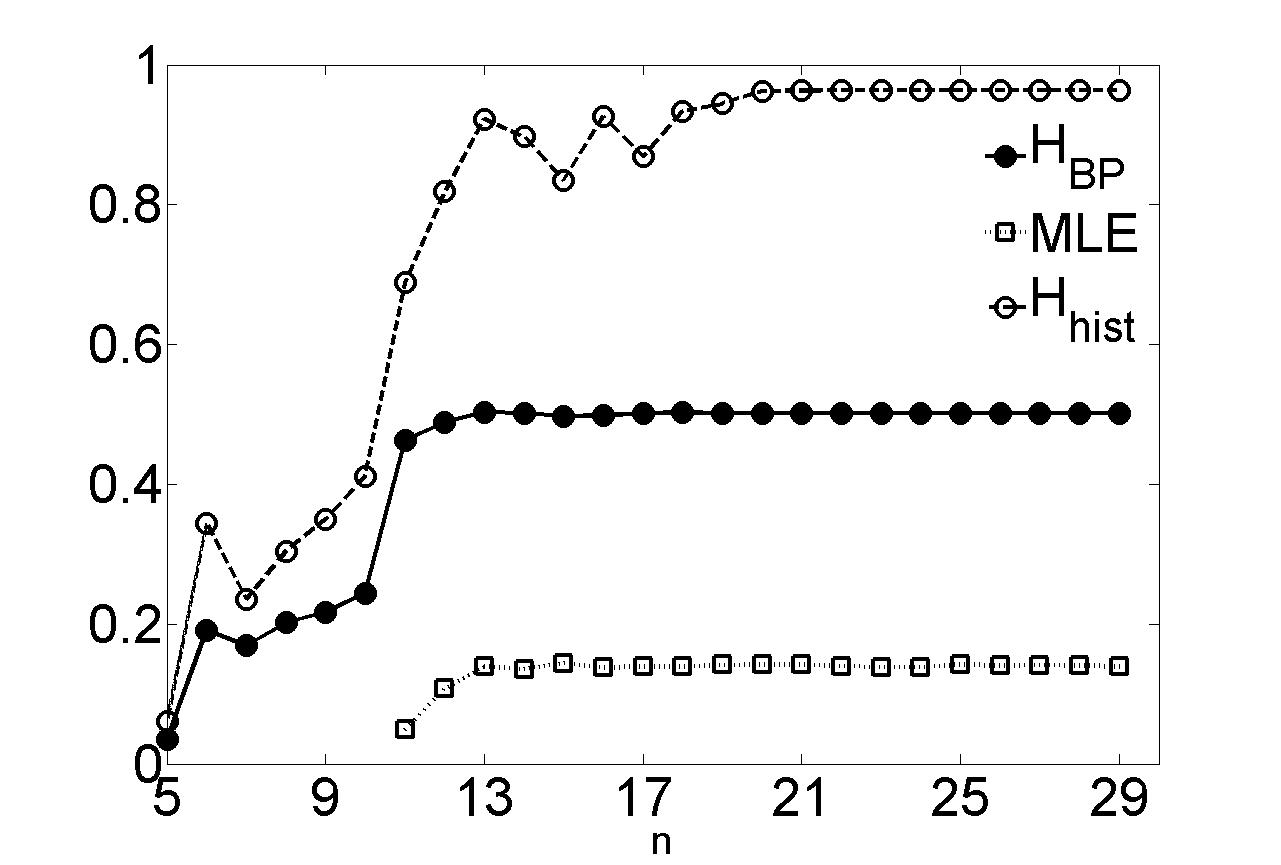
\includegraphics[width=0.9\columnwidth]{HBPHhist}\\
    \caption{Quantifiers $H_{BP}$ ,  $H_{hist}$ and $MLE$ as functions
     of the number of bits.}\label{fig:HBPHhist}
\end{figure}
%==================================================
%==================================================
\begin{figure}
    \centering
        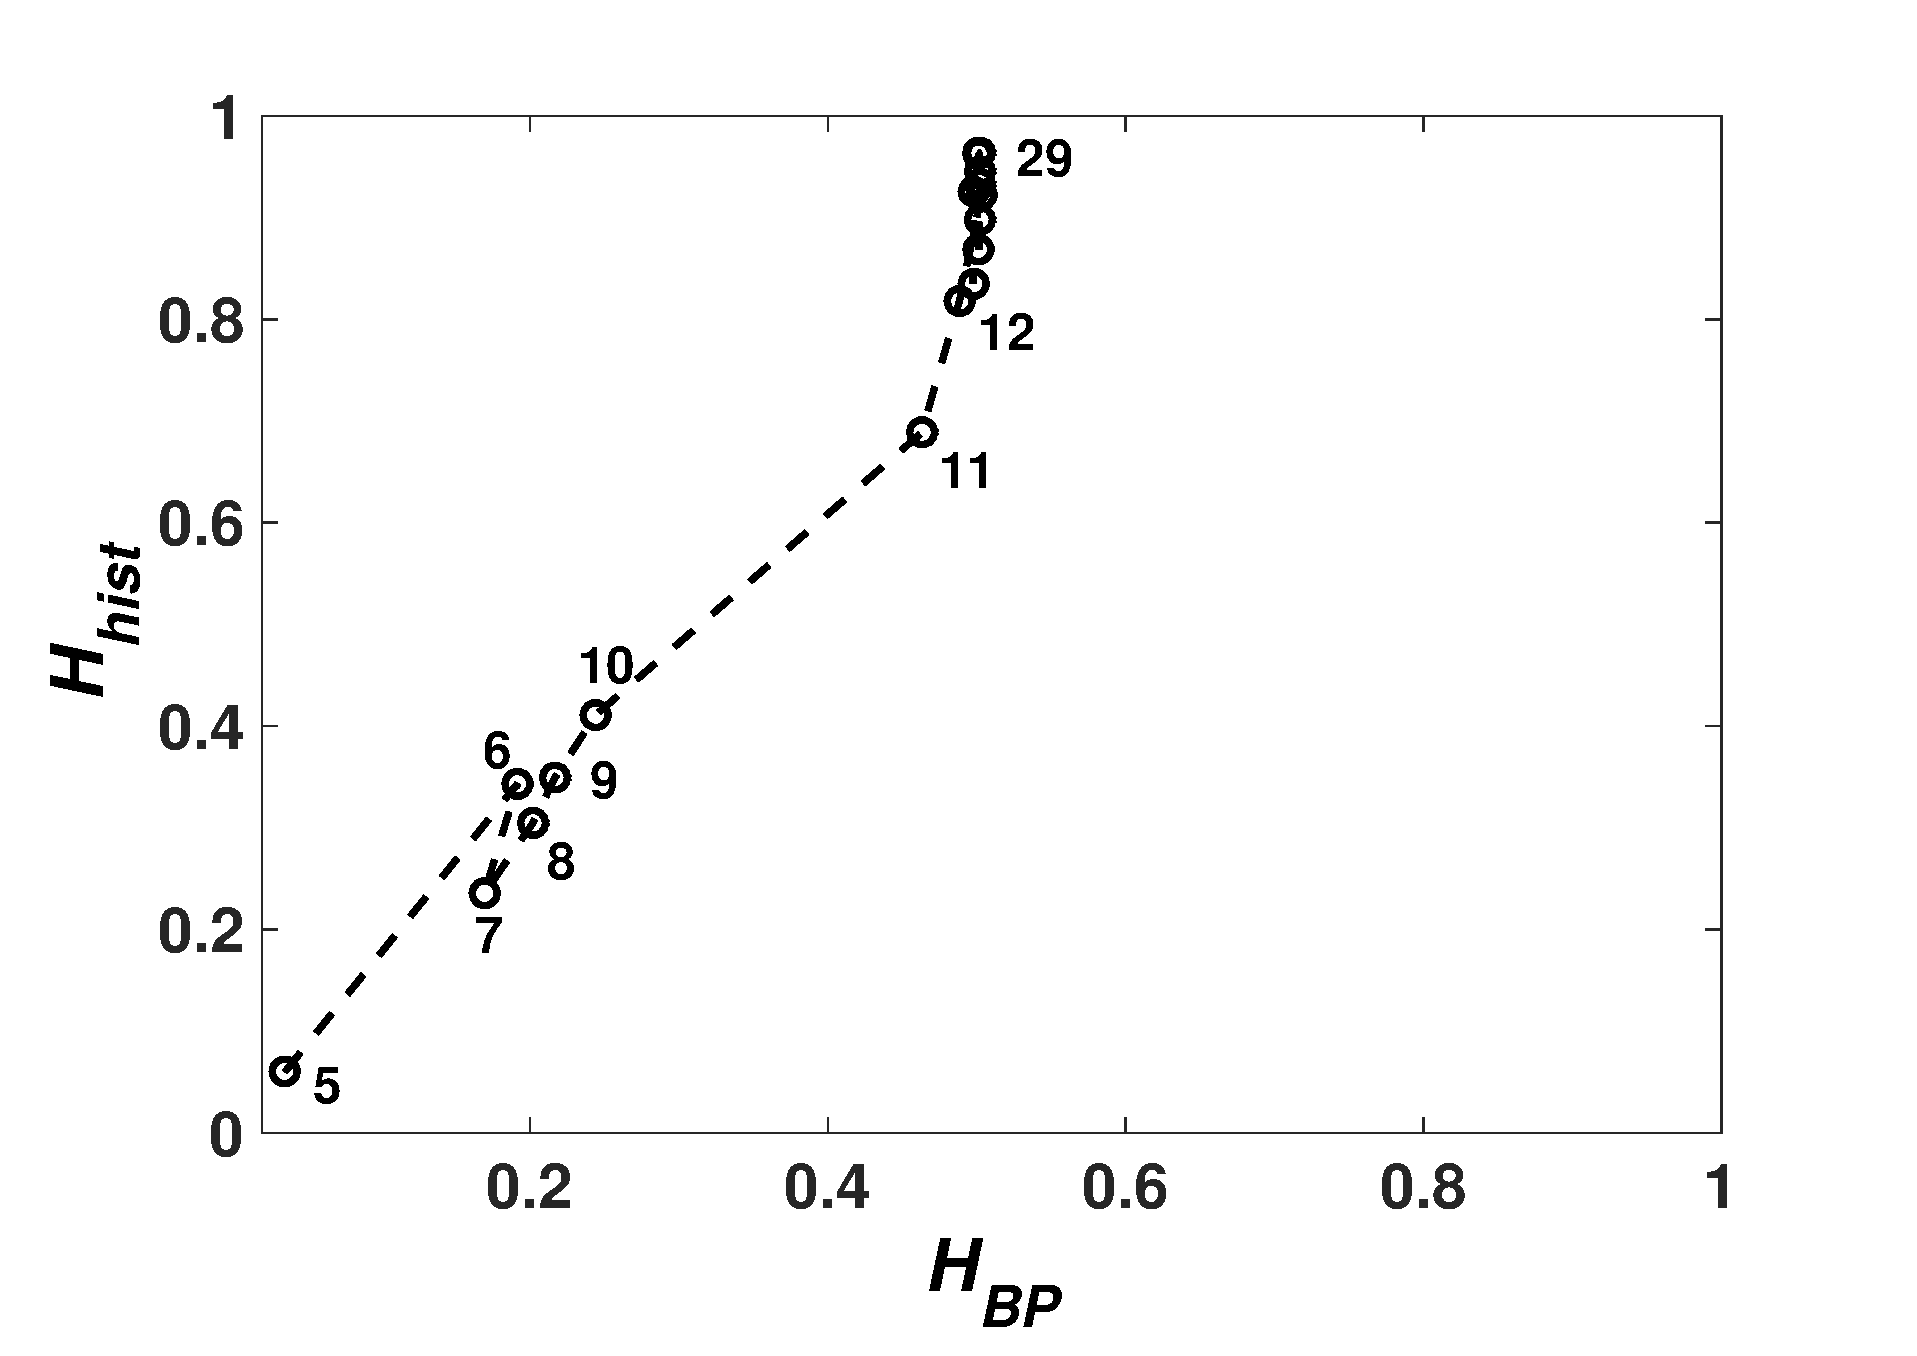
\includegraphics[width=0.9\columnwidth]{HBPvsHhist}\\
    \caption{Plane $H_{hist}$ - $H_{BP}$  for different number of bits. }\label{fig:HBPHhist}
\end{figure}
%==================================================
\end{document}
